
\documentclass[twoside]{report}

\usepackage{etoolbox}

\newdimen\Rwidth
\Rwidth=\textwidth


\usepackage[margin=.9in]{geometry}
\usepackage{probstat}
\usepackage{hyperref}
\usepackage[shownotes]{authNote}
\usepackage[answerdelayed,exercisedelayed,lastexercise]{problems}
\usepackage{longtable}

%\usepackage{tikz}

\usepackage[nogin]{Sweave}

\usepackage[Bjornstrup]{fncychap}
\usepackage{fancyvrb}
\usepackage{fancyhdr}
\pagestyle{fancy}
\fancyhf{}

%% Now begin customising things. See the fancyhdr docs for more info.

\renewcommand{\chaptermark}[1]{\thispagestyle{fancy}\markboth{{#1}}{}}
\renewcommand{\sectionmark}[1]{\markright{{#1}}{}}
%\renewcommand{\headrulewidth}{0pt}

\chead{}
\lhead[\sf \thepage]{\sf \leftmark}
\rhead[\sf \leftmark]{\sf \thepage}
\lfoot[\sf USCOTS 2011]{\sf Teaching Statistics With R}
\rfoot[\sf Teaching Statistics With R]{\sf USCOTS 2011}

\pagestyle{fancy}


%\usepackage{titlesec}
%\titleformat{\chapter}[block]{\huge \sf \bfseries }{\thechapter}{5mm}{}[] 



\def\R{{\sf R}}
\def\Rstudio{{\sf RStudio}}
\def\RStudio{{\sf RStudio}}
\def\term#1{\textbf{#1}}
\def\tab#1{{\sf #1}}

\usepackage{sfsect}
\usepackage{relsize}
%\usepackage{listings}

\def\myRuleColor{\color{black!50!white}}

\DefineVerbatimEnvironment{Sinput}{Verbatim} {fontsize=\small} 
\DefineVerbatimEnvironment{Soutput}{Verbatim} {fontsize=\small} 
%\DefineVerbatimEnvironment{Soutput}{Verbatim}{xleftmargin=5em} 
%\DefineVerbatimEnvironment{Scode}{Verbatim}{xleftmargin=2em} 
\fvset{listparameters={\setlength{\topsep}{0pt}}} 
\renewenvironment{Schunk}{\vspace{\topsep}}{\vspace{\topsep}} 

\definecolor{GrayBoxGray}{rgb}{0.94,0.95,0.95}
\definecolor{GrayBoxGray}{rgb}{0.97,0.98,0.95}
\colorlet{GrayBoxGray}{blue!10!black!10}
\colorlet{GrayBoxGray}{blue!7}
\makeatletter\newenvironment{graybox}{%
   \begin{lrbox}{\@tempboxa}\begin{minipage}{\Rwidth}}{\end{minipage}\end{lrbox}%
   \colorbox{GrayBoxGray}{\usebox{\@tempboxa}}
}\makeatother

\renewenvironment{Schunk}{

\noindent
\begin{graybox}}{\end{graybox}

}


\newlength{\tempfmlength}
\newsavebox{\fmbox}
\newenvironment{fmpage}[1]
     {
	 \medskip
	 \setlength{\tempfmlength}{#1}
	 \begin{lrbox}{\fmbox}
	   \begin{minipage}{#1}
		 \vspace*{.02\tempfmlength}
		 \hfill
	   \begin{minipage}{.95 \tempfmlength}}
		 {\end{minipage}\hfill
		 \vspace*{.015\tempfmlength}
		 \end{minipage}\end{lrbox}\fbox{\usebox{\fmbox}}
	 \medskip
	 }


\newenvironment{boxedText}[1][.98\textwidth]%
{%
\begin{center}
\begin{fmpage}{#1}
}%
{%
\end{fmpage}
\end{center}
}

\newenvironment{boxedTable}[2][tbp]%
{%
\begin{table}[#1]
  \refstepcounter{table}
  \begin{center}
\begin{fmpage}{.98\textwidth}
  \begin{center}
	\sf \large Box~\expandafter\thetable. #2
\end{center}
\medskip
}%
{%
\end{fmpage}
\end{center}
\end{table}		% need to do something about exercises that follow boxedTable
}



% indexing
\newcommand{\printindex}[1]{\relax}
\newcommand{\indexchap}[1]{\relax}
\usepackage{amsmidx}
\newcommand{\exampleidx}[1]{{\it #1}}
\newcommand{\defidx}[1]{{\bf #1}}
\newcommand{\mainidx}[1]{{\bf #1}}
\newcommand{\probidx}[1]{{{\underline{#1}}}}

\makeindex{Rindex}
\makeindex{mainIndex}
\newcommand{\Rindex}[1]{\index{Rindex}{#1@\texttt{#1}}}
\newcommand{\myindex}[1]{\index{mainIndex}{#1}}
\newcommand{\mathindex}[1]{\index{mainIndex}{$#1$}}

\newcommand{\cran}{\href{http://www.R-project.org/}{CRAN}}

\newcommand{\rterm}[1]{\textbf{#1}}


\title{Teaching Statistics with R}

\author{
Randall Pruim
\and
Nicholas Horton 
\and 
Daniel Kaplan 
}

\date{May, 2011}


\begin{document}
%%%%%%%%%%% comment this out if not using highlight %%%%%%%%%%%%%%%%%%%%%%
\newif\ifhweave
\ifdef{\hlcomment}{\hweavetrue}{\hweavefalse}
\ifhweave
\renewenvironment{Hchunk}%
{%
\vspace{0.5em}\noindent\begin{lrbox}{\highlightbox}%
\begin{minipage}[b]{\Rwidth}%
}%
{%
\end{minipage}%
\end{lrbox}%
%\fcolorbox{highlightBorder}{highlightBg}{\usebox{\highlightbox}}%
\fcolorbox{highlightBg}{highlightBg}{\usebox{\highlightbox}}%
\vspace{0.5em}}%

\renewcommand{\hlcomment}[1]{\textcolor[rgb]{0.4,0.4,0.3}{#1}}%
\fi
%%%%%%%%%%% end highlight specific stuff %%%%%%%%%%%%%%%%%%%%%%
\Rwidth=\textwidth

\parindent=0pt
\parskip=3mm

  % location of 
    % not sure this does anything unless we use pgfSweave
         % keep.source probably disables this
          % use pdf for graphics
  % remove blank lines at beginning and end 
  % keeps formatting from original; allows ? to work




\maketitle

\tableofcontents

\chapter*{Info for Authors}

\begin{center}
\it
We'll delete this later.
\end{center}

\section*{Document Creation}


This document was created
\today, using 
R version 2.12.2 (2011-02-25) 

\subsection*{Notes to Selves}

Notes for the authors can be included using \verb!\authNote{}!
\authNote{A note to the authors.}

Processed notes for the authors can be hidden using \verb!\authNoted{}!
\authNoted{A noted note to the authors.}

\subsection*{Some Style Guidelines}

\begin{enumerate}
\item
R Code
\begin{enumerate}
\item Use space after comma in argument lists 
\item No space around = in argument list
\item Use space around operators, \verb!<-! and \verb!->!
\item Casual comments (no need for caps)
\item When referring to functions in the text, add empty parens
(e.g., \verb!data()!) to make it clear that the object is a function.
\end{enumerate}
\item
Exercises
\begin{enumerate}
\item Use \verb!\begin{problem} ... \end{problem}! to define problems.
\item Use \verb!\begin{solution} ... \end{solution}! to define solutions.

This must be \emph{outside} the \verb!problem! environment and before 
the definition of the next problem.  Put it immediately after 
\verb!\end{problem}! to avoid confusion.

\item
Use \verb!\shipoutProblems! to display all problems queued up since the 
last \verb!shipoutProblems!.

\end{enumerate}

\item Examples

Do we want an example environment?  I've been using 
sectioning to indicate examples. --rjp

\end{enumerate}


\subsection*{The Makefile}
The document can be recompiled using
\begin{Schunk}
\begin{Sinput}
make all
\end{Sinput}
\end{Schunk}

which depends on 
\begin{itemize}
\item \verb!bin/sweave.sh! and 
\item \verb!bin/latexmk!.
\end{itemize}

Here is the current makefile:

\VerbatimInput[frame=single,numbers=left]{makefile}

\subsection*{R-forge svn}

The mosaic R-forge repository contains
\begin{itemize}
\item 
The \verb!.Rnw! files 
\item
the dependencies in \verb!bin/!
\item
\LaTeX\ dependencies in \verb!inputs/!  
\begin{itemize}
\item \verb!problems.sty! (for problems and solutions)
\item \verb!authNote.sty! (for author notes)
\item \verb!probstat.sty! (for some prob/stat macros)
\end{itemize}
You may need to set an environment variable to make \LaTeX\ look here.
\item
the \verb!cache/! and \verb!figures/! directories (so that \verb!make! can be used 
without complaint), but
\emph{not} their contents, which are generated by \verb!sweave!.

\item
screenshots and other images not generated by \verb!sweave! are in \verb!images/!
\end{itemize}


\chapter{Getting Started: The First Week With R }


  % location of 
    % not sure this does anything unless we use pgfSweave
         % keep.source probably disables this
          % use pdf for graphics
  % remove blank lines at beginning and end 
  % keeps formatting from original; allows ? to work


\section{Getting Students Familiar with R}

\subsection{Strategies}
\begin{enumerate}
\item
Start right away.

Do something with \R\ on day 1.  Have students do something by the end of week 1.


\item Illustrate frequently.

Have \R\ running every class period and use it as needed throughout the course so students
can see what \R\ does.  Preview topics by showing before asking students to do things.

\item
Teach \R\ as a programming language.

There is a bit of syntax to learn -- so teach it explicitly.
\begin{itemize}
\item
Capitalization (and spelling) matter
\item
Explain carefully (and repeatedly) the syntax of functions.
\item
Every object in \R\ has a type (class).  \emph{What type of thing is this?}
\item
Get students to think about what arguments are needed for functions:
\emph{What does this function need to know to do its job?}
\end{itemize}
Give more language details in higher level courses
\begin{itemize}
\item
More about \R\ classes
\item
User-defined functions
\item
Control structures
\end{itemize}

\item ``Less volume, more creativity."  [Mike McCarthy, head coach, Green Bay Packers]

Use a few methods frequently and students will learn how to use them well, flexibly, 
even creatively. 

Focus on a small number of data types: numerical vectors, character
strings, data frames.  

Not everything needs to be introduced from first principles.  For
instance, categorical variables are easily enough understood by
putting together simple concepts about character strings and vectors.

\item
Find a way to have computers available for tests.

It makes the test match the rest of the course and is a great motivator for students
to learn R.  It also changes what you can ask for and about on tests.

Randy began doing this when his students asked him if there was a way to use computers
during the test ``\emph{since that's how we do all the homework}."  He has students 
bring laptops to class.  

\item
Rethink your course.

If you have taught computer-free or computer-light courses in the past, you may need
to rethink some things.  With ubiquitous computing, some things disappear from your 
course:
\begin{itemize}
\item
Reading statistical tables.  

Does anyone still consult a table for values of $\sin$,
or $\log$?  Why use tables for statistical distributions?
\item
``Computational formulas".

Replace them with computation.  Teach only the most intuitive formulas. Focus on
how they lead to intuition and understanding, \emph{not} computation.

\item
(Most) hand calculations.

\end{itemize}
At the same time, other things become possible that were not before:
\begin{itemize}
\item
Large data sets
\item
Beautiful plots
\item
Simulation/randomization based methods
\item
Quick computations
\item
Increased focus on concepts rather than calculations
\end{itemize}
Get your students to think that using the computer is just part of how statistics is
done, rather than an add-on.  

\item
Anticipate computationally challenged students, but don't give in.

Some students pick up \R\ very easily.  In every course there will be a few students who
struggle.  Be prepared to help them, but don't  spend time listening to their complaints.
Focus on diagnosing what they don't know and how to help them ``get it''.

Tell students to copy and paste \R\ code and error messages into email when they
have trouble.  When you reply, explain how the error message helped you diagnose their
problem and help them generalize your solution to other situations.
\end{enumerate}

\subsection{Tactics}

\begin{enumerate}
\item
Introduce Graphics Early.


Do graphics very early, so that students see that they can get
impressive output from simple commands.  Try to break away from their
prior expectation that there is a "steep learning curve."

Accept the defaults -- don't worry about the niceties (good labels,
nice breaks on histograms, colors) too early.  Let them become
comfortable with the basic graphics commands and then play (make sure
it feels like play!) with fancying things up.  

Keep in mind that just because the graphs are easy to make on the computer doesn't 
mean your students understand how to read the graphs.  
Use examples that will
help students develop good habits for visualizing data.  Remember:

\begin{center}
\emph{
Students must learn to see before they can see to learn.}  -- R. Pruim
\end{center}

\item Introduce Sampling and Randomization Early.

Since sampling drives much of the logic of statistics, introduce the idea of a random sample very
early, and have students construct their own random samples.  The
phenomenon of a sampling distribution can be introduced in an
intuitive way, setting it up as a topic for later discussion and analysis.


\end{enumerate}

\section{ Examples for Early in the Course }
The remainder of this chapter has some of our favorite activities for early 
in the course.  


\subsection{Coins and Cups: The Lady Tasting Tea}

\begin{quote}
\emph{This section is a slightly modified version of a handout R. Pruim
has given Intro Stats students on Day 1 \underline{after} going through
the activity as a class discussion.  
}
\end{quote}


There is a famous story about a lady who claimed that
tea with milk tasted different depending on whether the milk was 
added to the tea or the tea added to the milk.
The story is famous because of the setting in which she made this claim.  
She was attending a party in Cambridge, England, in the $1920$s.
Also in attendance were a number of university dons and their wives.
The scientists in attendance scoffed at the woman and her claim.
What, after all, could be the difference?

\myindex{Fisher, R. A.}%
All the scientists but one, that is.  Rather than simply dismiss the 
woman's claim, he proposed that they decide how one 
should \emph{test} the claim.  The tenor of the conversation changed at 
this suggestion, and the scientists began to discuss how the claim should be 
tested.  Within a few minutes cups of tea with milk had been prepared and 
presented to the woman for tasting.

\iffalse
Let's take this simple example as a prototype for a statistical study.
What steps are involved?  
\begin{enumerate}
  \item Determine the question of interest.

	Just what is it we want to know?  It may take some effort to 
	make a vague idea precise.  The precise questions may not exactly
	correspond to our vague questions, and the very exercise of 
	stating the question precisely may modify our question.  Sometimes
	we cannot come up with any way to answer the question we really want
	to answer, so we have to live with some other question that is 
	not exactly what we wanted but is something we can study and will
	(we hope) give us some information about our original question.

	In our example this question seems fairly easy to state:
	Can the lady tell the difference between the two tea preparations?
	But we need to refine this question.  For example, are we 
	asking if she \emph{always} correctly identifies cups of tea
	or merely if she does better than we could do ourselves (by 
	guessing)?  

  \item 
	Determine the \term{population}. 
	\myindex{population}%

	Just who or what do we want to know about?  Are we only interested in
	this one woman or women in general or only women who claim to
	be able to distinguish tea preparations?

  \item
	Select \term{measurements}.

	We are going to need some data.  
	We get our data by making some measurements.
	These might be physical measurements with some device (like a ruler
	or a scale).
	But there are other sorts of measurements too, 
	like the answer to a question on a form.
	Sometimes it is tricky to figure out just what to measure.
	(How do we measure happiness or intelligence, for example?)
	Just how we do our measuring will have important consequences 
	for the subsequent statistical analysis.
	The recorded values of these measurements are called
	\term{variables} (because the values vary from one individual to another).

	In our example, a measurement may consist of recording for a given
	cup of tea whether the woman's claim is correct or incorrect.
	%it is milk-into-tea or tea-into-milk.

  \item
	Determine the \term{sample}.
	\myindex{sample}%

	Usually we cannot measure every individual in our population; we have 
	to select some to measure.  
	But how many and which ones?  
	These are important questions that must be answered.
	Generally speaking, bigger is better, but it is also more expensive.
	Moreover, no size is large enough if the sample is selected inappropriately.

	Suppose we gave the lady one cup of tea.  If she correctly identifies
	the mixing procedure, will we be convinced of her claim?  She might just
	be guessing; so we should probably have her taste more than one 
	cup.  Will we be convinced if she correctly identifies $5$ cups? $10$ cups?
	$50$ cups?

	What if she makes a mistake?  If we present her with $10$ cups and she
	correctly identifies $9$ of the $10$, what will we conclude?  
	\authNote{added A success rate of -- 2010-10-23}%
	A success rate of $90$\% is, it seems,
	much better than just guessing, and anyone can make a mistake now and then.
	But what if she correctly identifies $8$ out of $10$? $80$ out of $100$?
	
	And how should we prepare the cups?  Should we make $5$ each way?  
	\authNote{Left it as "and how" -- 2010-10-23}%
	Does it matter if we tell the woman that there are $5$ prepared 
	each way?
	Should we flip a coin to decide even if that means we might end 
	up with $3$ prepared one way and $7$ the other way?  
	Do any of these differences matter?

  \item
	Make and record the measurements.

	Once we have the design figured out, we have to do the legwork of 
	data collection.  This can be a time-consuming and tedious process.
	In the case of the lady tasting tea, the scientists decided to 
	present her with ten cups of tea which were quickly prepared.
	A study of public opinion may require many thousands of phone calls or 
	personal interviews.
	In a laboratory setting, each measurement might be the result 
	of a carefully performed laboratory experiment.

  \item Organize the data.

	Once the data have been collected, it is often necessary or useful
	to organize them.  Data are typically stored in spreadsheets or 
	in other formats that are convenient for processing with 
	statistical packages.  Very large data sets are often stored in 
	databases.  
	
	Part of the organization of the data may involve producing graphical and
	numerical summaries of the data.  These summaries may give us initial
	insights into our questions or help us detect errors that may have occurred
	to this point.

  \item Draw conclusions from data.

	Once the data have been collected, organized, and analyzed, we need
	to reach a conclusion.  
	Do we believe the woman's claim?  
	Or do we think she is merely guessing?  How sure are we that this
	conclusion is correct?

%	In Parts~\ref{part:inf1}--\ref{part:inf2} 
	Eventually we will
	learn a number of important and frequently used methods for 
	drawing inferences from data.  More importantly, we will learn
	the basic framework used for such procedures so that it should 
	become easier and easier to learn new procedures as we become 
	familiar with the framework.
	
	%How strongly do we believe it?  

  \item Produce a report.

		Typically the results of a statistical study are reported in 
		some manner.  This may be as a refereed article in an academic 
		journal, as an internal report to a company, or as a solution
		to a problem on a homework assignment.  These reports may themselves
		be further distilled into press releases, newspaper articles,
		advertisements, and the like.  The mark of a good report
		is that it provides the essential information about each 
		of the steps of the study.

		As we go along, we will learn some of the standard terminology and
		procedures that you are likely to see in basic statistical reports and 
		will gain a framework for learning more.  
\end{enumerate}

\fi

At this point, you may be wondering who the innovative scientist was and 
what the results of the experiment were.
\myindex{Fisher, R. A.}%
The scientist was R. A. Fisher, who first described this situation
as a pedagogical example in his 1925 book on 
statistical methodology \cite{Fisher:1925:Methods}.
Fisher developed statistical methods that are among the most
important and widely used methods to this day, and most of his 
applications were biological.
\nocite{Fisher:1970:Methods}%

You might also be curious about how the experiment came out.
How many cups of tea were prepared?  How many did the woman 
correctly identify?  What was the conclusion?

Fisher never says.  In his book he is interested in the method, not the 
particular results.  But let's suppose we decide to test the lady with
ten cups of tea.  
We'll flip a coin to decide which way to prepare the cups.  
If we flip a head, we will pour the milk in first; if tails, we 
put the tea in first.
Then we present the ten cups to the lady and have her state which ones she
thinks were prepared each way.  

It is easy to give her a score (9 out of 10, or 7 out of 10, or whatever
it happens to be).  It is trickier to figure out what to do with her score.
Even if she is just guessing and has no idea, she could get lucky and 
get quite a few correct -- maybe even all 10.  But how likely is that?

Let's try an experiment.  I'll flip 10 coins.  You guess which are heads and
which are tails, and we'll see how you do.  

$\vdots$

Comparing with your classmates, we will undoubtedly see that some 
of you did better and others worse.

Now let's suppose the lady gets 9 out of 10 correct.  That's not perfect,
but it is better than we would expect for someone who was just guessing.
On the other hand, it is not impossible to get 9 out of 10 just by guessing.
So here is Fisher's great idea:  Let's figure out how hard it is to get
9 out of 10 by guessing.  If it's not so hard to do, then perhaps that's 
just what happened, so we won't be too impressed with the lady's tea tasting
ability.  On the other hand, if it is really unusual to get 9 out of 10 
correct by guessing, then we will have some evidence that she must 
be able to tell something.

But how do we figure out how unusual it is to get 9 out of 10 just by 
guessing?  We'll learn another method later, but for now, let's just 
flip a bunch of coins and keep track.  If the lady is just guessing, she 
might as well be flipping a coin.

So here's the plan.  We'll flip 10 coins.  We'll call the heads correct 
guesses and the tails incorrect guesses.  Then we'll flip 10 more coins,
and 10 more, and 10 more, and \dots.  That would get pretty tedious.
Fortunately, computers are good at tedious things, so we'll let the computer 
do the flipping for us.

The \verb!rflip()! function can flip one coin

\begin{Schunk}
\begin{Sinput}
> require(mosaic)
> rflip()
\end{Sinput}
\begin{Soutput}
Flipping 1 coins [ Prob(Heads) = 0.5 ] ...

H

Result: 1 heads.
\end{Soutput}
\end{Schunk}
or a number of coins
\begin{Schunk}
\begin{Sinput}
> rflip(10)
\end{Sinput}
\begin{Soutput}
Flipping 10 coins [ Prob(Heads) = 0.5 ] ...

H T T T H T H H H T

Result: 5 heads.
\end{Soutput}
\end{Schunk}
%and show us the results.

Typing \verb!rflip(10)! a bunch of times is almost as tedious as 
flipping all those coins.   But it is not too hard to 
tell \R\ to \verb!do()! this a bunch of times.
\begin{Schunk}
\begin{Sinput}
> do(3) * rflip(10)
\end{Sinput}
\begin{Soutput}
   n heads tails
1 10     5     5
2 10     4     6
3 10     5     5
\end{Soutput}
\end{Schunk}

Let's get \R\ to \verb!do()! it for us 10,000 times and make 
a table of the results.


\begin{Schunk}
\begin{Sinput}
> random.ladies <- do(10000) * rflip(10)
\end{Sinput}
\end{Schunk}
\vspace{-5mm}

\begin{Schunk}
\begin{Sinput}
> table(random.ladies$heads)
\end{Sinput}
\begin{Soutput}
   0    1    2    3    4    5    6    7    8    9   10 
   5  102  467 1203 2048 2470 2035 1140  415  108    7 
\end{Soutput}
\begin{Sinput}
> perctable(random.ladies$heads)     # display table using percentages
\end{Sinput}
\begin{Soutput}
    0     1     2     3     4     5     6     7     8     9    10 
 0.05  1.02  4.67 12.03 20.48 24.70 20.35 11.40  4.15  1.08  0.07 
\end{Soutput}
\end{Schunk}

We can display this table graphically using a plot called a \term{histogram}.
\vspace{-8mm}
\begin{center}
\begin{Schunk}
\begin{Sinput}
> histogram(~heads, random.ladies, 
+ 	breaks=-.5 + (0:11)
+ 	)
\end{Sinput}
\end{Schunk}
\includegraphics{figures/fig-lady-hist}
\end{center}

You might be surprised to see that the number of correct guesses
is exactly 5 (half of the 10 tries) only 
0\%
of the time.  But most of the results are quite close to 5 correct.
67\% of the results are 
4, 5, or 6, for example.
And 90\% of the results 
are  between 3 and 7 (inclusive).
But getting 8 correct is a bit unusual, and getting 9 or 10 correct is even 
more unusual.  

So what do we conclude?  It is possible that the lady could get 9 or 10 correct
just by guessing, but it is not very likely (it only happened in about
0.1\% of our simulations). 
So \emph{one of two things must be true}:
\begin{itemize}
\item The lady got unusually ``lucky", or 
\item The lady is not just guessing.
\end{itemize}

Although Fisher did not say how the experiment came out, others have reported
that the lady correctly identified all 10 cups!
\cite{salsburg}




\section{Graphical and Numerical Summaries}

\section{Going Multivariate Early: Galton's Data}

Using Francis Galton's data, investigate how an adult child's height depends on the height of the parents.  Is
it mainly the father's height, mainly the mother's?  What's the role
of the child's gender, e.g., do boys inherit height from the father
and girls from the mother?  Make this a research question for the students.  

RJP added some plots here just to see what the data looked like.  
Keep/delete/modify at your discretion.

\begin{center}
\begin{Schunk}
\begin{Sinput}
> xyplot(height ~ father+mother| sex, galton, type=c('p','r'), auto.key=T, alpha=.6)
\end{Sinput}
\end{Schunk}
\includegraphics{figures/fig-galton}
\begin{Schunk}
\begin{Sinput}
> xyplot(father~mother, galton, type=c('p','r'), auto.key=T, alpha=.3)
\end{Sinput}
\end{Schunk}
\includegraphics{figures/fig-galton-parents}
\end{center}


\chapter{Simulation Based Inference}


  % location of 
    % not sure this does anything unless we use pgfSweave
         % keep.source probably disables this
          % use pdf for graphics
  % remove blank lines at beginning and end 
  % keeps formatting from original; allows ? to work


\section{\texttt{mosaic} randomization widgets}

\section{Examples}
\subsection{Lady Tasting Tea}
If you don't use the Lady Tasting Tea as a course starter, you can use it as 
an introduction to testing a proportion.

\subsection{Golfballs in the Yard}



\section{Bootstrap?}

Do any of us do bootstrap in intro courses?  Other courses?  Do we want to include this?
Robin Lock is big on bootstrap.  Do we need any bootstrap tools in the \verb!mosaic! 
package?

Danny responds: We already have good-enough bootstrap tools in the
package: \texttt{do} and \texttt{resample}.  I don't do bootstrapping
early in the course, but I do talk about sampling variability from day
1.  Later on, I introduce bootstrapping as a way to simulate sampling
variability without having to collect more data.


\chapter{Taking Advantage of the Internet}


  % location of 
    % not sure this does anything unless we use pgfSweave
         % keep.source probably disables this
          % use pdf for graphics
  % remove blank lines at beginning and end 
  % keeps formatting from original; allows ? to work


\section{Google Docs and \RStudio}

\section{Sharing in \RStudio}

\section{Other Ways to Make Data Available Online}

\section{Data Mining Activities}
\subsection{What percentage of Earth is Covered with Water?}
We can estimate the proportion of the world covered with water by randomly 
sampling points on the globe and inspecting them using GoogleMaps.

First, let's do a sample size computation.  Suppose we want to 
estimate (at the 95\% confidence level) this proportion with $\pm 5$\%.
There are several ways to estimate the necessary sample size, including
algebraically solving
\[
(1.96) \sqrt{ \hat p (1-\hat p) /n} = 0.05
\]
for $n$ given some estimated value of $p$.  The \verb!uniroot()! function
can solve this sort of thing numerically.  Here we take an approach 
that looks at a table of values of $n$ and $\hat p$ and margin of error.
\begin{Schunk}
\begin{Sinput}
> n <- seq(50,500, by=50)
> p.hat <- seq(.5, .9, by=0.10)
> margin_of_error <- function(n, p, conf.level=.95) { 
+ 	-qnorm( (1-conf.level)/2) * sqrt( p * (1-p) / n ) 
+ }
> outer(n, p.hat, margin_of_error) -> tbl
> colnames(tbl) <- p.hat
> rownames(tbl) <- n
> tbl
\end{Sinput}
\begin{Soutput}
           0.5        0.6        0.7        0.8        0.9
50  0.13859038 0.13579029 0.12702018 0.11087231 0.08315423
100 0.09799820 0.09601823 0.08981683 0.07839856 0.05879892
150 0.08001519 0.07839856 0.07333514 0.06401216 0.04800912
200 0.06929519 0.06789514 0.06351009 0.05543615 0.04157711
250 0.06197950 0.06072726 0.05680515 0.04958360 0.03718770
300 0.05657929 0.05543615 0.05185577 0.04526343 0.03394757
350 0.05238224 0.05132390 0.04800912 0.04190579 0.03142934
400 0.04899910 0.04800912 0.04490842 0.03919928 0.02939946
450 0.04619679 0.04526343 0.04234006 0.03695744 0.02771808
500 0.04382613 0.04294066 0.04016731 0.03506090 0.02629568
\end{Soutput}
\end{Schunk}
From this it appears that a sample size of approximately 300--400 will get
us the accuracy we desire.  A class of students can easily generate
this much data in a matter of minutes if each student inspects 10--20 maps.
The example below assumes a sample size of 10 locations per student.
This can be adjusted depending on the number of students and the desiered
margin of error.

\begin{enumerate}
\item Generate 10 random locations.

\begin{Schunk}
\begin{Sinput}
> positions <- rgeo(10); positions
\end{Sinput}
\begin{Soutput}
           lat        lon
1  -33.1662372  -42.42110
2   45.4895488 -135.10702
3  -20.9049703   57.67713
4  -47.6480390  -59.97332
5    0.5762188  -58.90692
6  -30.0055680  -76.58094
7  -31.9636897  -21.37841
8    5.1491013  -46.46827
9   16.5316968  103.48692
10 -53.5463879  -24.52795
\end{Soutput}
\end{Schunk}

\item
Open a GoogleMap centered at each position.

\begin{Schunk}
\begin{Sinput}
> googleMap(pos=positions, mark=TRUE)
\end{Sinput}
\end{Schunk}
You may need to turn off pop-up block for this to work smoothly.

\item
For each map, record whether the center is located in water or on land.  \verb!mark=TRUE!
is used to place a marker at the center of the map which is helpful for locations that are close to 
the coast.  
\begin{center}
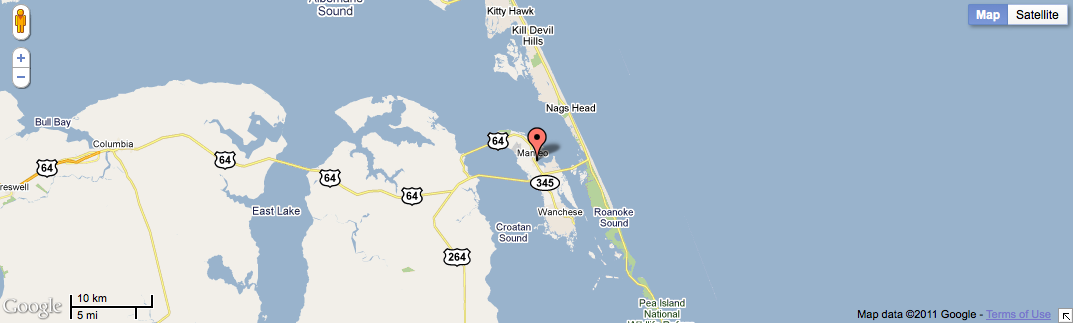
\includegraphics[width=.8\textwidth]{images/google-water1}
\end{center}
You can zoom in or out to get a better look.
\begin{center}
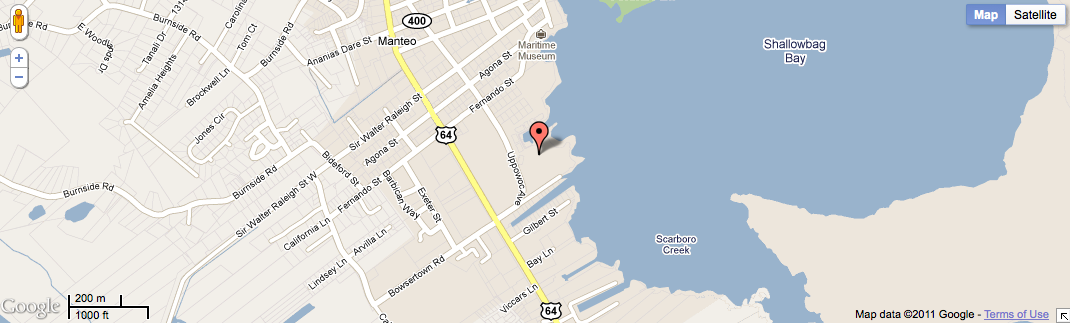
\includegraphics[width=.8\textwidth]{images/google-water2}
\end{center}


\item
Record your data in a GoogleForm at 

\begin{center}
\url{https://spreadsheets.google.com/viewform?formkey=dGREcUR6YjRLSWFTWVpNNXA5ZUZ1TXc6MQ}

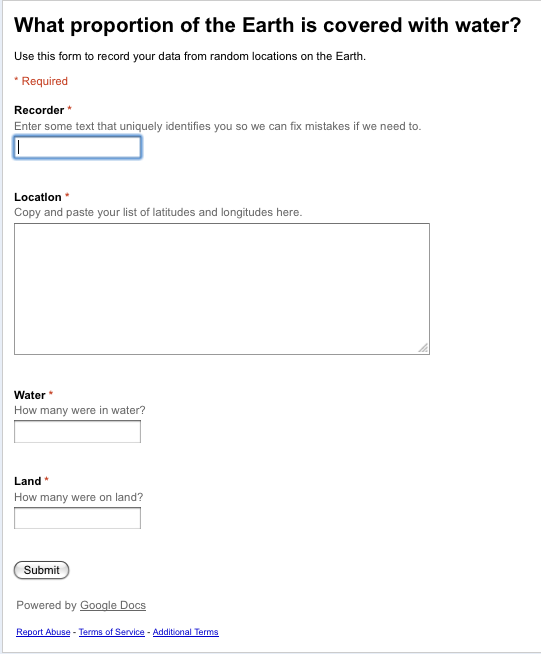
\includegraphics[width=.4\textwidth]{images/googleForm-water}
\end{center}

For the latitude and longitude information, simply copy and paste the output of 
\begin{Schunk}
\begin{Sinput}
> positions
\end{Sinput}
\end{Schunk}
\item
After importing the data from Google, it is simple to sum the counts across the class.


\begin{Schunk}
\begin{Sinput}
> sum(Water$Water)
\end{Sinput}
\begin{Soutput}
[1] 215
\end{Soutput}
\begin{Sinput}
> sum(Water$Land)
\end{Sinput}
\begin{Soutput}
[1] 85
\end{Soutput}
\end{Schunk}

Then use your favorite method of analysis, perhaps \verb!binom.test()!.

\begin{Schunk}
\begin{Sinput}
> interval(binom.test(215,300))
\end{Sinput}
\begin{Soutput}
Method: Exact binomial test

probability of success 
             0.7166667 

95% confidence interval: 
0.662036 0.7669599
\end{Soutput}
\end{Schunk}
\end{enumerate}


\subsection{Roadless America}

The \verb!rgeo()! can also sample within a latitude longitude ``rectangle".
This allows us to sample subsets of the globe.  In this activity we will estimate 
the proportion of the continental United States that is within 1 mile of a road.

\begin{enumerate}
\item
Generate a random sample of locations in a box containing the continental United States.
Some of these points may be in Canada, Mexico, an ocean or a major lake.  These 
will be discarded from our sample before making our estimate.
\begin{Schunk}
\begin{Sinput}
> positions <- rgeo(10, lonlim=c(-125,-65), latlim=c(25,50)); positions
\end{Sinput}
\begin{Soutput}
        lat        lon
1  40.49504  -84.32582
2  37.89567 -118.64393
3  29.91783 -117.66907
4  37.09653  -73.96205
5  42.93143 -112.48634
6  27.55399 -117.77189
7  39.59000  -91.24735
8  31.02972 -109.40219
9  29.81856 -122.67036
10 25.18305  -91.40336
\end{Soutput}
\end{Schunk}

\item
Open a GoogleMap centered at each position.  This time we'll zoom in a bit and add 
a circle of radius 1 to our map.

\begin{Schunk}
\begin{Sinput}
> googleMap(pos=positions, mark=TRUE, zoom=12, radius=1)
\end{Sinput}
\end{Schunk}


\begin{center}
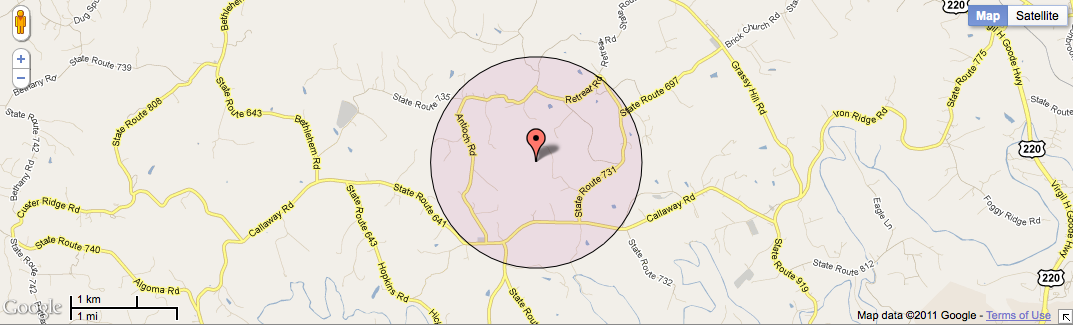
\includegraphics[width=.8\textwidth]{images/google-roadless}
\end{center}
You may need to turn off pop-up block for this to work smoothly.
\item
For each map, record whether the center is close (to a road), far (from a road), water, or foreign.
You may need to zoom in or out a bit to figure this out.

\end{enumerate}

\subsection{Variations on the Google Maps theme}

There are many other quantities one could estimate using these tools.  For example:
\begin{enumerate}
\item
What proportion of you home state is within $m$ miles of a lake?  (The choice of $m$ may depend upon
your state of interest.)
\item
Use two proportion procedures  or chi-squared tests to compare states or continents.  
Do all continents have roughly the same proportion of land withing $m$ miles of water (for some $m$)?
Are Utah and Arizona equally roadless?

\item
In more advanced classes: What is the average distance to the nearest lake (in some region)?
By using concentric circles, one could estimate this from discretized data indicating, for example,
whether the nearest lake is within 1/2 mile, between 1/2 mile and 1 mile, between 1 mile and 2 miles,
between 2 miles, and 4 miles, between 4 miles and 10 miles, or more than 10 miles away.  It may be 
interesting to discuss what sort of model should be used for distances from random locations to lakes.
(It probably isn't normally distributed.)
\authNote{Is this example too complicated?}%
\end{enumerate}

\subsection{Zillow}
Nick 



\chapter{Multivariate Statistics -- Early?}


  % location of 
    % not sure this does anything unless we use pgfSweave
         % keep.source probably disables this
          % use pdf for graphics
  % remove blank lines at beginning and end 
  % keeps formatting from original; allows ? to work


\section{Danny's Favorite Example}

\section{Danny's Second Favorite Example}




\chapter{The Core of a Traditional Course}

  % location of 
    % not sure this does anything unless we use pgfSweave
         % keep.source probably disables this
          % use pdf for graphics
  % remove blank lines at beginning and end 
  % keeps formatting from original; allows ? to work



\section{Inference for Proportions}

\section{Inference for Means}

\section{Chi-Squared Tests}

\subsection{Dealing with Categorical Data}

\section{Linear Models: Regression and ANOVA}


\include{Chap-MoreExamples}



  % location of 
    % not sure this does anything unless we use pgfSweave
         % keep.source probably disables this
          % use pdf for graphics
  % remove blank lines at beginning and end 
  % keeps formatting from original; allows ? to work



\chapter{Calculus in R}



\appendix

\chapter{Getting Started with R}


  % location of 
    % not sure this does anything unless we use pgfSweave
         % keep.source probably disables this
          % use pdf for graphics
  % remove blank lines at beginning and end 
  % keeps formatting from original; allows ? to work


\begin{quote}
\emph{This is a lightly modified version of a handout RJP used with his 
Intro Stats students Spring 2011.}
\end{quote}

\label{app:StartingR}

\section{Welcome to \R\ and \Rstudio}

\R\ is a system for statistical computation and graphics.  We will use \R\ in this course 
for several reasons:
\begin{enumerate}
\item \R\ is open-source and freely available for Mac, PC, and Linux machines.
\item \R\ is user-extensible and user extensions can easily be made available to others.
\item \R\ is commercial quality.  It is the package of choice for many statisticians and those
who use statistics frequently.  
\item \R\ is becoming very popular with biologists, especially in certain
sub-disciplines, like genetics.  Articles in research journals such as \textit{Science} often
include links to the \R\ code used for the analysis and graphics presented.
\item
\R\ is very powerful.  Furthermore, it is gaining new features every day.  New statistical 
methods are often available first in \R.
\end{enumerate}

\Rstudio\ provides access to \R\ in a web browser.  The URL is
\begin{center}
\url{http://beta.rstudio.org/}
\end{center}
You shouldbe able to log in using your Calvin ID (\texttt{myname@calvin.edu})  
and KnightVision password.  Once you have logged in, you will see something like 
Figure~\ref{fig:Rstudio-bigview}.

\begin{figure}
\begin{center}
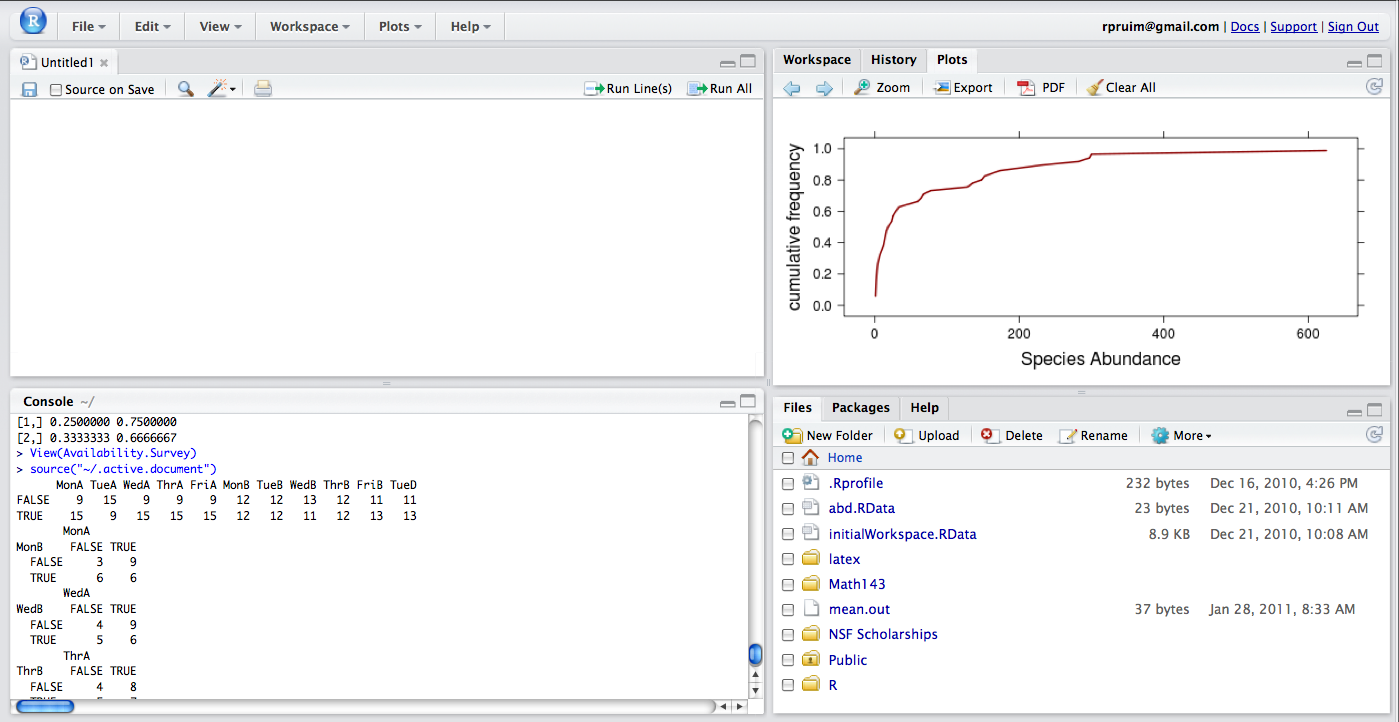
\includegraphics[width=.75\textwidth]{images/RStudio-bigview}
\end{center}
\caption{Welcome to \Rstudio.}
\label{fig:Rstudio-bigview}%
\end{figure}

Notice that \Rstudio\ divides its world into four panels.  Several of the panels
are further subdivided into multiple tabs.
The console panel is where we type commands that \R\ will execute. 

\begin{problem}
Calculate the natural logarithm (log base $e$) and base 10 logarithm of 12,345.
Copy-and-paste your \R\ code into your Word document.  
Be sure to use a fixed-width font (like Courier) when you display \R\ code.  This will
(1) make it clear that you are displaying \R\ input or output, and (2) keep things aligned 
properly.
\end{problem}

\pagebreak
\section{Using R as a Calculator}
\R\ can be used as a calculator.  Try typing the following commands in the console panel.

\begin{Schunk}
\begin{Sinput}
> 5 + 3
\end{Sinput}
\begin{Soutput}
[1] 8
\end{Soutput}
\begin{Sinput}
> 15.3 * 23.4
\end{Sinput}
\begin{Soutput}
[1] 358.02
\end{Soutput}
\begin{Sinput}
> sqrt(16)
\end{Sinput}
\begin{Soutput}
[1] 4
\end{Soutput}
\end{Schunk}
You can save values to named variables for later reuse

\begin{Schunk}
\begin{Sinput}
> product = 15.3 * 23.4       # save result
> product                     # show the result
\end{Sinput}
\begin{Soutput}
[1] 358.02
\end{Soutput}
\begin{Sinput}
> product <- 15.3 * 23.4      # <- is assignment operator, same as =
> product                     
\end{Sinput}
\begin{Soutput}
[1] 358.02
\end{Soutput}
\begin{Sinput}
> 15.3 * 23.4 -> newproduct   # -> assigns to the right
> newproduct
\end{Sinput}
\begin{Soutput}
[1] 358.02
\end{Soutput}
\begin{Sinput}
> .5 * product                # half of the product
\end{Sinput}
\begin{Soutput}
[1] 179.01
\end{Soutput}
\begin{Sinput}
> log(product)                # (natural) log of the product
\end{Sinput}
\begin{Soutput}
[1] 5.880589
\end{Soutput}
\begin{Sinput}
> log10(product)              # base 10 log of the product
\end{Sinput}
\begin{Soutput}
[1] 2.553907
\end{Soutput}
\begin{Sinput}
> log(product,base=2)         # base 2 log of the product
\end{Sinput}
\begin{Soutput}
[1] 8.483896
\end{Soutput}
\end{Schunk}

The semi-colon can be used to place multiple commands on one line.  
One frequent use of this is to save and print a value all in one go:

\begin{Schunk}
\begin{Sinput}
> 15.3 * 23.4 -> product; product    # save result and show it
\end{Sinput}
\begin{Soutput}
[1] 358.02
\end{Soutput}
\end{Schunk}


\subsection*{Four Things to Know About \R}
\begin{enumerate}
\Rwidth=6.25in
\item \R\ is case-sensitive

If you mis-capitalize something in \R\ it won't do what you want.

\item 
Functions in \R\ use the following syntax:

\begin{Schunk}
\begin{Sinput}
> functionname( argument1, argument2, ... )
\end{Sinput}
\end{Schunk}
\vspace{-5mm}
\begin{itemize}
\item The arguments are \underline{always} \emph{surrounded by (round) parentheses} and 
\emph{separated by commas}.

Some functions (like \verb!data()!) 
have no required arguments, but you still need the parentheses.

\item
If you type a function name without the parentheses, you will see the \emph{code} for that
function -- which probably isn't what you want at this point.
\end{itemize}
\item
TAB completion and arrows can improve typing speed and accuracy.

If you begin a command and hit the TAB key, \R\ will show you a list of possible ways to 
complete the command.  If you hit TAB after the opening parenthesis of a function, it will show you
the list of arguments it expects.  The up and down arrows can be used to retrieve past commands.
\item
If you see a \verb!+! prompt, it means \R\ is waiting for more input.

Often this means that you have forgotten a closing parenthesis or made some other
syntax error.  If you have messed up and just want to get back to the normal plot,
hit the escape key and start the command fresh.
\end{enumerate}

\section{R packages}

In addition to its core features, \R\ provides many more features through a (large) number 
of packages.  To use a package, it must be installed (one time), and loaded (each session).
A number of packages are already available in \Rstudio.  
The \tab{Packages} tab in \Rstudio\ will show you the list of installed packages and indicate
which of these are loaded.

\begin{center}
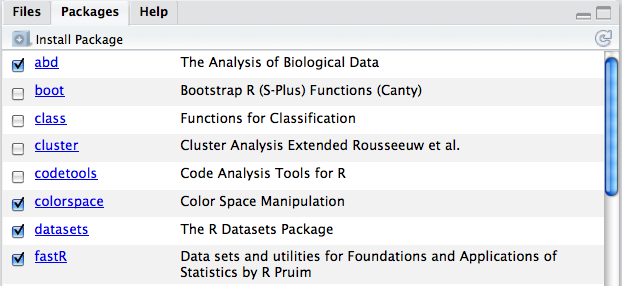
\includegraphics[width=.55\textwidth]{images/RStudio-packages}
\end{center}

%(A similar thing is true for the stand-alone versions of \R.)

Here are some packages we will use frequently in this course:
\begin{itemize}
\item \verb!lattice!  (for graphics; this will always be installed in \R)
\item \verb!Hmisc!    (a package with some nice utilities; available on CRAN)
\item \verb!vcd!      (a package for visualizing categorical data; available on CRAN)
\item \verb!fastR!    (a package with some nice utilities; available on CRAN)
\item \verb!abd!      (a package with data and utilities for our textbook; available on CRAN)
\end{itemize}
There may be others that we use from time to time as well.  You should install
\verb!Hmisc!, \verb!vcd!, \verb!fastR!, \verb!abd!, and \verb!mosaic! 
(in that order) the first time you use \R\ 
so that they are always available to you.
You can install these packages 
by clicking on the ``Install Package" button and following the directions
or by using the following commands:

\begin{Schunk}
\begin{Sinput}
> install.packages('Hmisc')           # note the quotation marks 
> install.packages('vcd')
> install.packages('fastR')
> install.packages('abd')
> install.packages('mosaic')
\end{Sinput}
\end{Schunk}

Once these are installed, you can load them by checking the box in the 
\tab{Packages} tab or by using the commands

\begin{Schunk}
\begin{Sinput}
> require(lattice)
> require(Hmisc)
> require(vcd)
> require(fastR)
> require(abd)
> require(mosaic)
\end{Sinput}
\end{Schunk}

\begin{problem}
Install and load the following packages:
\verb!Hmisc!,
\verb!vcd!,
\verb!fastR!, and 
\verb!abd!.
Make sure \verb!lattice! is also loaded (no need to install it, it is already installed).
\end{problem}


\section{Data}
\subsection{Data in Packages}
Many packages contain data sets.  You can see a list of all data sets in all loaded packages
using 

\begin{Schunk}
\begin{Sinput}
> data()
\end{Sinput}
\end{Schunk}

The \verb!abd! package contains data sets from our text,
\textit{The Analysis of Biological Data}.  The \verb!findData()! function
can help you determine the correct name for the data set you are looking
for.

\begin{Schunk}
\begin{Sinput}
> findData('human')         # all data sets with 'human' in the name
\end{Sinput}
\begin{Soutput}
               name chapter    type number sub
24 HumanGeneLengths       4 Example      1    
43    HumanBodyTemp      11 Example      3    
\end{Soutput}
\end{Schunk}

\begin{Schunk}
\begin{Sinput}
> findData(2)               # all data sets in chapter 2
\end{Sinput}
\begin{Soutput}
                   name chapter    type number sub
1            TeenDeaths       2 Example      1   a
2           DesertBirds       2 Example      1   b
3        SockeyeFemales       2 Example      1   c
4       GreatTitMalaria       2 Example      3    
5            Hemoglobin       2 Example      4    
6               Guppies       2 Example      5   a
7                  Lynx       2 Example      5   b
8     EndangeredSpecies       2 Problem      6    
9       ShuttleDisaster       2 Problem     10    
10          Convictions       2 Problem     16    
11 ConvictionsAndIncome       2 Problem     17    
12            Fireflies       2 Problem     18    
13     NeotropicalTrees       2 Problem     23    
\end{Soutput}
\end{Schunk}

Typically you can use data sets by simply typing their names.  But if you have already
used that name for something or need to refresh the data after making some changes you no longer
want, you can explicitly load the data using the \verb!data()! function with the name of the 
data set you want.

\begin{Schunk}
\begin{Sinput}
> data(iris)
\end{Sinput}
\end{Schunk}

\subsection{Data Frames}

Data sets are usually stored in a special structure called a \term{data frame}.

\begin{boxedText}
Data frames have a 2-dimensional structure.  
\medskip
\begin{itemize}
\item 
Rows correspond to 
\term{observational units} (people, animals, plants, or other objects we
are collecting data about).
\item
Columns correspond to \term{variables} (measurements collected on each 
observational unit).
\end{itemize}
\end{boxedText}

We'll talk later about how to get your own data into \R.  For now we'll use 
some data that comes with \R\ and is all ready for you to use.
The \verb!iris! data frame contains 5 \term{variables} measured for each
of 150 iris plants (the observational units).  
The \verb!iris! data set is included with the default \R\ installation.  
(Technically, it is located in a package called \verb!datasets!  which is always available.)

There are several ways we can get some idea about what is in the \verb!iris! data frame.

\begin{Schunk}
\begin{Sinput}
> str(iris)
\end{Sinput}
\begin{Soutput}
'data.frame':	150 obs. of  5 variables:
 $ Sepal.Length: num  5.1 4.9 4.7 4.6 5 5.4 4.6 5 4.4 4.9 ...
 $ Sepal.Width : num  3.5 3 3.2 3.1 3.6 3.9 3.4 3.4 2.9 3.1 ...
 $ Petal.Length: num  1.4 1.4 1.3 1.5 1.4 1.7 1.4 1.5 1.4 1.5 ...
 $ Petal.Width : num  0.2 0.2 0.2 0.2 0.2 0.4 0.3 0.2 0.2 0.1 ...
 $ Species     : Factor w/ 3 levels "setosa","versicolor",..: 1 1 1 1 1 1 1 1 1 1 ...
\end{Soutput}
\end{Schunk}

\begin{Schunk}
\begin{Sinput}
> summary(iris)
\end{Sinput}
\begin{Soutput}
  Sepal.Length    Sepal.Width     Petal.Length    Petal.Width          Species  
 Min.   :4.300   Min.   :2.000   Min.   :1.000   Min.   :0.100   setosa    :50  
 1st Qu.:5.100   1st Qu.:2.800   1st Qu.:1.600   1st Qu.:0.300   versicolor:50  
 Median :5.800   Median :3.000   Median :4.350   Median :1.300   virginica :50  
 Mean   :5.843   Mean   :3.057   Mean   :3.758   Mean   :1.199                  
 3rd Qu.:6.400   3rd Qu.:3.300   3rd Qu.:5.100   3rd Qu.:1.800                  
 Max.   :7.900   Max.   :4.400   Max.   :6.900   Max.   :2.500                  
\end{Soutput}
\end{Schunk}

\begin{Schunk}
\begin{Sinput}
> head(iris)
\end{Sinput}
\begin{Soutput}
  Sepal.Length Sepal.Width Petal.Length Petal.Width Species
1          5.1         3.5          1.4         0.2  setosa
2          4.9         3.0          1.4         0.2  setosa
3          4.7         3.2          1.3         0.2  setosa
4          4.6         3.1          1.5         0.2  setosa
5          5.0         3.6          1.4         0.2  setosa
6          5.4         3.9          1.7         0.4  setosa
\end{Soutput}
\end{Schunk}
In interactive mode, you can also try

\begin{Schunk}
\begin{Sinput}
> View(iris)
\end{Sinput}
\end{Schunk}
to see the data or 

\begin{Schunk}
\begin{Sinput}
> ?iris
\end{Sinput}
\end{Schunk}
to get the documentation about for the data set.

%\subsection{Getting at the Variables}
Access to an individual variable in a data frame uses the \verb!$! operator in
the following syntax:

\begin{Schunk}
\begin{Sinput}
> dataframe$variable
\end{Sinput}
\end{Schunk}

For example,

\begin{Schunk}
\begin{Sinput}
> iris$Sepal.Length
\end{Sinput}
\begin{Soutput}
  [1] 5.1 4.9 4.7 4.6 5.0 5.4 4.6 5.0 4.4 4.9 5.4 4.8 4.8 4.3 5.8 5.7 5.4 5.1 5.7 5.1 5.4 5.1 4.6
 [24] 5.1 4.8 5.0 5.0 5.2 5.2 4.7 4.8 5.4 5.2 5.5 4.9 5.0 5.5 4.9 4.4 5.1 5.0 4.5 4.4 5.0 5.1 4.8
 [47] 5.1 4.6 5.3 5.0 7.0 6.4 6.9 5.5 6.5 5.7 6.3 4.9 6.6 5.2 5.0 5.9 6.0 6.1 5.6 6.7 5.6 5.8 6.2
 [70] 5.6 5.9 6.1 6.3 6.1 6.4 6.6 6.8 6.7 6.0 5.7 5.5 5.5 5.8 6.0 5.4 6.0 6.7 6.3 5.6 5.5 5.5 6.1
 [93] 5.8 5.0 5.6 5.7 5.7 6.2 5.1 5.7 6.3 5.8 7.1 6.3 6.5 7.6 4.9 7.3 6.7 7.2 6.5 6.4 6.8 5.7 5.8
[116] 6.4 6.5 7.7 7.7 6.0 6.9 5.6 7.7 6.3 6.7 7.2 6.2 6.1 6.4 7.2 7.4 7.9 6.4 6.3 6.1 7.7 6.3 6.4
[139] 6.0 6.9 6.7 6.9 5.8 6.8 6.7 6.7 6.3 6.5 6.2 5.9
\end{Soutput}
\end{Schunk}
shows the contents of the \verb!Sepal.Length! variable.  But this isn't very useful 
for a large data set.  We would prefer to compute numerical or graphical summaries.
We'll do that shortly.

\subsection{Using Your Own Data}
\Rstudio\ will help you import you own data.  To do so use the ``Import Dataset" 
button in the \tab{Workspace} tab.  You can load data from text files, from the web, or from
google spreadsheets.   

%\subsubsection*{From Google Spreadsheets}

\textbf{From Google.}
The easiest of these is the Google spreadsheets option: Just click, select
your spreadsheet, choose a name, and you're done.

%\subsubsection*{From Excel}
\textbf{From Excel},
you need to follow a 3-step process:
\begin{enumerate}
\item
Save your Excel worksheet as a csv file.
\item
Upload (in the \tab{Files} tab) your csv file to the server, where you can create folders and store
files in your personal account.  
(To share things with others: Put the files in your Public folder.  
Read the\texttt{AboutPublic.txt} file in that folder for directions.)
\item
Now import ``from a text file'' in the \tab{Workspace} tab.
\end{enumerate}

In either case, be sure to do the following:
\begin{itemize}
\item Choose good variables names.
\item Put your variables names in the first row.
\item Use each subsequent row for one observational unit.
\item Give the resulting data frame a good name.
\end{itemize}
\authNote{I moved Danny's Simple Relational Database suggestion
to \ref{sec:manipulatingData}.
I don't think I would use a grade/courses example for students nor that
I would introduce \verb!merge()! \emph{et al} to newbies right away.
My goal was to have this appendix look like something that I would give
to students as is in the first week.
In any case, I agree that we should have a section on this somewhere.
[RJP]
}%

\begin{problem}
Enter the following small data set in an Excel or Google spreadsheet and import the 
data into \Rstudio.

\begin{center}
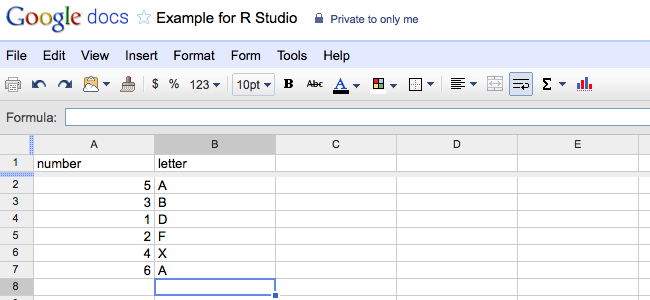
\includegraphics[width=.5\textwidth]{images/GoogleSpreadsheet}
\end{center}

You can import directly from Google.  From Excel, save the file as a csv and
import that (as a text file) into \Rstudio.  Name the data frame \texttt{JunkData}.
Copy and paste the results of 

\begin{Schunk}
\begin{Sinput}
> JunkData
\end{Sinput}
\end{Schunk}
into your report.  (Remember to use a fixed width font like Courier for all \R\ input and 
output.)
\end{problem}


\section{Summarizing Data}

\subsection{A Few Numerical Summaries}
\R\ includes functions that compute a wide range of numerical and graphical summaries.  
Most of the numerical summaries already familiar to you have obvious names.  
Here are a few examples.  (If you don't know what some of these -- like IQR -- are, don't worry;
we'll be discussing them soon.)

\begin{Schunk}
\begin{Sinput}
> mean(iris$Sepal.Length)
\end{Sinput}
\begin{Soutput}
[1] 5.843333
\end{Soutput}
\begin{Sinput}
> median(iris$Sepal.Length)
\end{Sinput}
\begin{Soutput}
[1] 5.8
\end{Soutput}
\begin{Sinput}
> sd(iris$Sepal.Length)
\end{Sinput}
\begin{Soutput}
[1] 0.8280661
\end{Soutput}
\begin{Sinput}
> quantile(iris$Sepal.Length)
\end{Sinput}
\begin{Soutput}
  0%  25%  50%  75% 100% 
 4.3  5.1  5.8  6.4  7.9 
\end{Soutput}
\end{Schunk}

The \verb!favstats()! function in the \verb!abd! package computes several numerical 
summaries all at once.

\begin{Schunk}
\begin{Sinput}
> require(abd)             # if you haven't already loaded the abd package
> favstats(iris$Sepal.Length)
\end{Sinput}
\begin{Soutput}
   median       IQR      mean        sd       var 
5.8000000 1.3000000 5.8433333 0.8280661 0.6856935 
\end{Soutput}
\end{Schunk}

Here's something a little fancier.

\begin{Schunk}
\begin{Sinput}
> summary(Sepal.Length ~ Species, data=iris, fun=favstats)
\end{Sinput}
\begin{Soutput}
Sepal.Length    N=150

+-------+----------+---+------+-----+--------+---------+---------+
|       |          |N  |median|IQR  |mean    |sd       |var      |
+-------+----------+---+------+-----+--------+---------+---------+
|Species|setosa    | 50|5.0   |0.400|5.006000|0.3524897|0.1242490|
|       |versicolor| 50|5.9   |0.700|5.936000|0.5161711|0.2664327|
|       |virginica | 50|6.5   |0.675|6.588000|0.6358796|0.4043429|
+-------+----------+---+------+-----+--------+---------+---------+
|Overall|          |150|5.8   |1.300|5.843333|0.8280661|0.6856935|
+-------+----------+---+------+-----+--------+---------+---------+
\end{Soutput}
\end{Schunk}
(Note: This requires installation of two add-on packages: \verb!Hmsic! 
and \verb!abd!.)

\begin{problem}
What is the average (mean) \emph{width} of the sepals in the \verb!iris! data set?
\end{problem}

\begin{problem}
Determine the average (mean) sepal width for each of the three species in the \verb!iris! data set.
\end{problem}

\subsection{Lattice Graphics}

There are several ways to make graphs in \R.  I like to use a system called
\verb!lattice! graphics.  The first step for using \verb!lattice! is to
load the \verb!lattice! package using the check box in the \tab{Packages} tab or using
the following command:

\begin{Schunk}
\begin{Sinput}
> require(lattice)
\end{Sinput}
\end{Schunk}
\verb!lattice! plots make use of a \term{formula interface}:

\begin{Schunk}
\begin{Sinput}
> plotname( y ~ x | z, data=dataname, groups=grouping_variable, ...)
\end{Sinput}
\end{Schunk}
\begin{itemize}
\item
Our most common plots have the following names:
\begin{itemize}
\item \verb!dotPlot! (notice the capital P; \verb!dotplot()! does something different)
\item \verb!histogram!
\item \verb!bwplot!
\item \verb!xyplot!
\end{itemize}
\item
\verb!x! is the name of the variable that is plotted along the horizontal 
($x$) axis.
\item
\verb!y! is the name of the variable that is plotted along the vertical ($y$) 
axis.  (For some plots, this slot is empty because \R\ computes these values
from the values of \verb!x!.)
\item
\verb!z! is a conditioning variable used to split the plot into 
multiple subplots called \term{panels}.
\item
\verb!grouping_variable! is used to display different groups differently
(different colors or symbols, for example) within the same panel.
\item
\verb!...! There are many additional arguments to these functions that let you
control just how the plots look.  (But we'll focus on the basics for now.)
\end{itemize}

%\subsection*{Some Examples}

\subsection{Dot plots: \texttt{dotPlot()}}

A dot plot represents each value of a quantitative variable with a dot.  The values
are rounded a bit so that the dots line up neatly, and dots are stacked up into little
towers when the data values cluster near each other.

For a dot plot, the \verb!y! component of the formula is empty since we let \R\
calculate that for us.

\begin{center}
\begin{Schunk}
\begin{Sinput}
> dotPlot(~Sepal.Length, data=iris, n=20)   # n=20 gives us approximately 20 towers
\end{Sinput}
\end{Schunk}
\includegraphics{figures/fig-iris-dotPlot}
\end{center}
We can use a conditional variable to give us separate dot plots for each species.

\begin{Schunk}
\begin{Sinput}
> dotPlot(~Sepal.Length|Species, data=iris, n=20)
\end{Sinput}
\end{Schunk}
\begin{center}
\includegraphics{figures/fig-iris-dotPlot-condB}
\end{center}

\subsection{Histograms: \texttt{histogram()}}

Histograms are a lot like dot plots, but the towers of dots are replaced by a vertical bar.
Again the \verb!y! component of the formula is empty since we let \R\
compute the heights of the bars for us.
\begin{center}
\begin{Schunk}
\begin{Sinput}
> histogram(~Sepal.Length, data=iris, n=20)       # n= 20 gives approx. 20 bars
\end{Sinput}
\end{Schunk}
\includegraphics{figures/fig-iris-histogram}
\end{center}
We can use a conditional variable to give us separate histograms for each species.

\begin{center}
\begin{Schunk}
\begin{Sinput}
> histogram(~Sepal.Length|Species, data=iris, n=20)
\end{Sinput}
\end{Schunk}
\includegraphics{figures/fig-iris-histogram-cond}
\end{center}


In lattice lingo, the three subplots are called panels and the 
labels at the top are called strips.  (Strips can be placed on the left side if you 
prefer.)


\subsection{Boxplots:  \texttt{bwplot()}}

Boxplots are made pretty much the same way as histograms:
\begin{center}
\begin{Schunk}
\begin{Sinput}
> bwplot(~Sepal.Length, data=iris)
\end{Sinput}
\end{Schunk}
\includegraphics{figures/fig-iris-bwplot}
\end{center}

We can use conditioning as we did for histograms:

\begin{center}
\begin{Schunk}
\begin{Sinput}
> bwplot(~Sepal.Length|Species, data=iris)
\end{Sinput}
\end{Schunk}
\includegraphics{figures/fig-iris-bwplot-cond}
\end{center}

\vspace{-8mm}

But there are betters ways to do this.
This is better, but the species names run into each other.
\begin{center}
\begin{Schunk}
\begin{Sinput}
> bwplot(Sepal.Length~Species, data=iris)
\end{Sinput}
\end{Schunk}
\includegraphics{figures/fig-iris-bwplot-2d}
\end{center}

We could fix that run-together text by using abbreviated names or rotating the
labels 45 or 90 degrees.  Instead of those solutions, we can also just reverse the roles
of the horizontal and vertical axes.
\begin{center}
\begin{Schunk}
\begin{Sinput}
> bwplot(Species ~ Sepal.Length, data=iris)
\end{Sinput}
\end{Schunk}
\includegraphics{figures/fig-iris-bwplot-2dh}
\end{center}

\vspace{-12mm}

%\pagebreak

\subsection{Scatterplots: \texttt{xyplot()}}

Scatterplots are made with \verb!xyplot()!.  The formula interface is very natural for this.  
Just remember that the ``$y$ variable'' comes first.  (Its label is also farther left on 
the plot, if that helps you remember.)
\begin{center}
\begin{Schunk}
\begin{Sinput}
> xyplot(Sepal.Length ~ Sepal.Width, data=iris)
\end{Sinput}
\end{Schunk}
\includegraphics{figures/fig-iris-xyplot}
\end{center}

Again, we can use conditioning to make a panel for each species.
\begin{center}
\begin{Schunk}
\begin{Sinput}
> xyplot(Sepal.Length ~ Sepal.Width|Species, data=iris)
\end{Sinput}
\end{Schunk}
\includegraphics{figures/fig-iris-xyplot-cond}
\end{center}


Even better (for this example), we can use the \verb!groups! argument to indicate the different species using
different symbols on the same panel.
\begin{center}
\begin{Schunk}
\begin{Sinput}
> xyplot(Sepal.Length ~ Sepal.Width, groups=Species, data=iris)
\end{Sinput}
\end{Schunk}
\includegraphics{figures/fig-iris-xyplot-groups}
\end{center}

\subsection{Saving Your Plots}

There are several ways to save plots, but the easiest is probably the following:
\begin{enumerate}
\item
In the \tab{Plots} tab, click the ``Export'' button.
\item
Copy the image to the clipboard using right click.
\item
Go to your Word document and paste in the image.
\item
Resize or reposition your image in Word as needed.
\end{enumerate}

\subsection{A Few Bells and Whistles}
There are lots of arguments that control how these plots look.  Here are just a few examples.

\subsubsection{auto.key}
It would be useful to have a legend for the previous plot.   \verb!auto.key=TRUE! 
turns on a simple legend.  (There are ways to have more control, if you need it.)
\begin{center}
\begin{Schunk}
\begin{Sinput}
> xyplot(Sepal.Length ~ Sepal.Width, groups=Species, data=iris, 
+ 	auto.key=TRUE)   
\end{Sinput}
\end{Schunk}
\includegraphics{figures/fig-iris-xyplot-key}
\end{center}

\subsubsection{alpha, cex}
Sometimes it is nice to have elements of a plot be partly transparent.  When such
elements overlap, they get darker, showing us where data are ``piling up."
Setting the \verb!alpha! argument to a value between 0 and 1 controls the degree 
of transparency: 1 is completely opaque, 0 is invisible.
The \verb!cex! argument controls ``character expansion" and can be used to make the 
plotting ``characters" larger or smaller by specifying the scaling ratio.
\begin{center}
\begin{Schunk}
\begin{Sinput}
> xyplot(Sepal.Length ~ Sepal.Width, groups=Species, data=iris, 
+ 	auto.key=list(columns=3),
+ 	alpha=.5,
+ 	cex=1.3)   
\end{Sinput}
\end{Schunk}
\includegraphics{figures/fig-iris-xyplot-alpha}
\end{center}

\vspace{-8mm}
\subsubsection*{main, sub, xlab, ylab}

You can add a title or subtitle, or change the default labels of the axes.
\begin{center}
\begin{Schunk}
\begin{Sinput}
> xyplot(Sepal.Length ~ Sepal.Width, groups=Species, data=iris, 
+ 	main="Some Iris Data",
+ 	sub="(R. A. Fisher analysized this data in 1936)",
+ 	xlab="sepal width (cm)",
+ 	ylab="sepal length (cm)",
+ 	alpha=.5,        
+ 	auto.key=list(columns=3))   
\end{Sinput}
\end{Schunk}
\includegraphics{figures/fig-iris-xyplot-text}
\end{center}

\subsubsection{trellis.par.set()}
Default settings for lattice graphics are set using 
\verb!trellis.par.set()!.
Don't like the default font sizes?  You can change to a 7 point (base) font using

\begin{Schunk}
\begin{Sinput}
> trellis.par.set(fontsize=list(text=7))    # base size for text is 7 point 
\end{Sinput}
\end{Schunk}


Nearly every feature of a lattice plot can be controlled: fonts, colors,
symbols, line thicknesses, colors, etc.
Rather than describe them all here, we'll mention only that groups of these settings 
can be collected into a theme.  \verb!show.settings()! will show you what the theme looks like.

\begin{Schunk}
\begin{Sinput}
> trellis.par.set(theme=col.whitebg())      # a theme in the lattice package
> show.settings()
\end{Sinput}
\end{Schunk}
\includegraphics{figures/fig-themes-whitbg}

\begin{Schunk}
\begin{Sinput}
> trellis.par.set(theme=col.abd())          # a theme in the abd package
> show.settings()
\end{Sinput}
\end{Schunk}
\includegraphics{figures/fig-themes-abd}

\begin{Schunk}
\begin{Sinput}
> trellis.par.set(theme=col.mosaic())        # a theme in the mosaic package
> show.settings()
\end{Sinput}
\end{Schunk}
\includegraphics{figures/fig-themes-mosaic}

\begin{Schunk}
\begin{Sinput}
> trellis.par.set(theme=col.mosaic(bw=TRUE)) # black and white version of previous theme
> show.settings()
\end{Sinput}
\end{Schunk}
\includegraphics{figures/fig-themes-mosaicbw}

\begin{Schunk}
\begin{Sinput}
> trellis.par.set(theme=col.abd())          # back to the abd theme
> trellis.par.set(fontsize=list(text=9))    # and back to a 10 point font
\end{Sinput}
\end{Schunk}

\begin{problem}
The \verb!Jordan8687! data set (in the \verb!fastR! package) contains the number 
of points Michael Jordan scored in each game of the 1986--87 season.  
\begin{enumerate}
\item
Make a histogram of this data.  Add an appropriate title.
\item
How would you describe the shape of the distribution?
\item
In approximately what percentage of his games, did Michael Jordan score less than 20 points?
More than 50?
(You may want to add \verb!breaks=seq(0,70,by=5)! to your command to neaten up
the bins.)
\end{enumerate}
\end{problem}

\begin{problem}
Cuckoos lay their eggs in the nests of other birds.  Is the size of cuckoo eggs different
in different host species nests?  The \verb!cuckoo! data set (in \verb!fastR!)
contains data from a study attempting to answer this question.
\begin{enumerate}
\item
When were these data collected?  (Use \verb!?cuckoo! to get information about the data set.)
\item
What are the units on the length measurements?
\item
Make side-by-side boxplots of the length of the eggs by species.
\item
Calculate the mean length of the eggs for each host species.
\item
What do you think?  Does it look like the size is differs among the different host
species?  Refer to your \R\ output as you answer this question.
(We'll learn formal methods to investigate this later in the semester.)
\end{enumerate}
\vspace{-5mm}
\end{problem}

%\subsection{Bar Charts and Pie Charts}
\subsection{Tabulating Categorical Data}
The \verb!Trematodes! data set contains data from an experiment to see if
fish infected with a certain parasite are more likely to be eaten by birds 
(because they swim closer to the surface of the water).  Highly infected, 
lightly infected, and uninfected fish were placed in an outdoor tank that 
was open to foraging birds.  For each fish, the researchers recorded its
infection status and whether it had been eaten.

\begin{Schunk}
\begin{Sinput}
> require(abd)
> head(Trematodes,3)
\end{Sinput}
\begin{Soutput}
    infection.status eaten
1         uninfected   yes
2         uninfected    no
2.1       uninfected    no
\end{Soutput}
\end{Schunk}

\subsubsection{Making Frequency and Contingency Tables with \texttt{xtabs()}}
Categorical variables are  often summarized in a table.  
\R\ can make a table for a categorical variable using \verb!xtabs()!.

\begin{Schunk}
\begin{Sinput}
> xtabs(~infection.status, Trematodes)
\end{Sinput}
\begin{Soutput}
infection.status
      high      light uninfected 
        46         45         50 
\end{Soutput}
\begin{Sinput}
> xtabs(~eaten,Trematodes)
\end{Sinput}
\begin{Soutput}
eaten
 no yes 
 93  48 
\end{Soutput}
\end{Schunk}

%\subsubsection{Cross-Tabulation with \texttt{xtabs()}}
We can make a \term{cross-table} 
(also called a \term{contingency table} or a \term{two-way table}) 
summarizing this data with \verb!xtabs()!.  This is often a more useful view of 
data with two categorical variables.

\begin{Schunk}
\begin{Sinput}
> xtabs( ~ infection.status + eaten, Trematodes)
\end{Sinput}
\begin{Soutput}
                eaten
infection.status no yes
      high        9  37
      light      35  10
      uninfected 49   1
\end{Soutput}
\end{Schunk}

\subsubsection*{Entering Tables by Hand}

Because categorical data is so easy to summarize in a table, 
often the frequency or contingency tables are given instead.
You can enter these tables manually as follows:


\begin{Schunk}
\begin{Sinput}
> myinfection <- c( high=46, light=46, uninfected=50); myinfection
\end{Sinput}
\begin{Soutput}
      high      light uninfected 
        46         46         50 
\end{Soutput}
\end{Schunk}

\label{R:make-xtabs}%
\begin{Schunk}
\begin{Sinput}
> mycrosstable <- rbind(                        # bind row-wise
+                   high = c(no=9, yes=37),     # note labels
+                   light = c(35,10),           # don't need to relabel columns
+                   uninfected = c(49,1)        # note commas throughout
+ 			)
\end{Sinput}
\end{Schunk}

\begin{Schunk}
\begin{Sinput}
> mycrosstable
\end{Sinput}
\begin{Soutput}
           no yes
high        9  37
light      35  10
uninfected 49   1
\end{Soutput}
\end{Schunk}
Replacing \verb!rbind()! with \verb!cbind()! will allow you to give the data
column-wise instead.

\subsection{Graphing Categorical Data}

%\subsubsection{Bar charts and pie charts}
%We won't use these plots often, in part because summary tables are already a good
%way to understand the data.  
The \verb!lattice! function \verb!barchart! can display these tables as barcharts.
\begin{center}
\begin{Schunk}
\begin{Sinput}
> barchart(xtabs(~infection.status, Trematodes))
\end{Sinput}
\end{Schunk}
\includegraphics{figures/fig-barchart1a}
\begin{Schunk}
\begin{Sinput}
> barchart(xtabs(~infection.status, Trematodes), horizontal=FALSE)  # vertical bars
\end{Sinput}
\end{Schunk}
\includegraphics{figures/fig-barchart2a}
\end{center}

\vspace{-6mm}
If the data are already summarized, we can make our bar charts without using
\verb!xtabs()! (Figure~\ref{fig:TeenDeaths-barchart}).

\begin{Schunk}
\begin{Sinput}
> barchart(cause~deaths,TeenDeaths,horizontal=TRUE)
\end{Sinput}
\end{Schunk}
\begin{figure}
\begin{center}
\includegraphics{figures/fig-TeenDeaths-2}
\end{center}
\vspace{-8mm}
\caption{\texttt{barchart(cause\~{}deaths,TeenDeaths,horizontal=TRUE)}}
\label{fig:TeenDeaths-barchart}%
\end{figure}

\iffalse
Statisticians almost never use pie charts.  They are harder to read than bar charts.
The \verb!lattice! package doesn't even include a function to make pie charts.
But the \verb!pie()! function from the \verb!graphics!  package can make these
plots if you absolutely have to have one:

\begin{Schunk}
\begin{Sinput}
> pie(table(Trematodes$infection.status))
> pie(table(Trematodes$eaten))
\end{Sinput}
\end{Schunk}
\fi
\iffalse
\begin{center}
\includegraphics{figures/fig-pie1}
\includegraphics{figures/fig-pie2}
\end{center}
These are probably the last pie charts you will see in this class.
\fi


%\subsubsection{Mosaic plots}

Just as bar charts and pie charts are used to display the distribution
of one categorical variable,  mosaic plots can do the same for cross tables.
\verb!mosaic()! (from the \verb!vcd! package) is not a \verb!lattice! plot, 
but it does use a similar formula interface.  %(See Figure~\ref{fig:mosaic}.)

\begin{Schunk}
\begin{Sinput}
> require(vcd)                              # load the visualing categorical data package
> mosaic(~ infection.status + eaten, Trematodes)
\end{Sinput}
\begin{Soutput}
                 eaten no yes
infection.status             
high                    9  37
light                  35  10
uninfected             49   1
\end{Soutput}
\end{Schunk}


Alternatively, we can send \verb!mosaic()! the output of \verb!xtabs()!:
\begin{center}
\begin{Schunk}
\begin{Sinput}
> mosaic(xtabs(~ infection.status + eaten, Trematodes))
\end{Sinput}
\begin{Soutput}
                 eaten no yes
infection.status             
high                    9  37
light                  35  10
uninfected             49   1
\end{Soutput}
\end{Schunk}
\end{center}

%\vspace{-12mm}
\begin{figure}[h]
\begin{center}
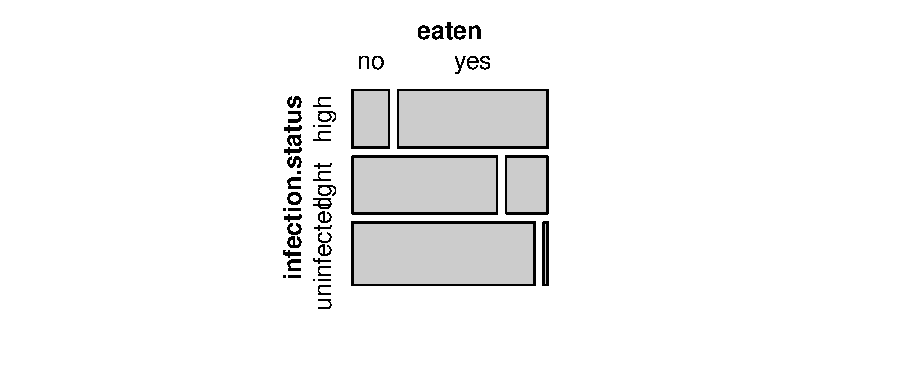
\includegraphics[width=.65\textwidth]{images/fig-mosaic1}
\end{center}
%\caption{\texttt{mosaic(\~{} infection.status + eaten, Trematodes)}}
%\label{fig:mosaic}
\end{figure}

\vspace{-12mm}
Or we can send our own hand-made table (although the output isn't quite as nice without some
extra effort we won't discuss just now):
\begin{center}
\begin{Schunk}
\begin{Sinput}
> mosaic(mycrosstable)
\end{Sinput}
\end{Schunk}
\end{center}

\iffalse
\vspace{-5mm}
Want it the other way around like the other plots?  You can build your table the other way or you can transpose 
the one you have with \verb!t()!:
\begin{center}
\begin{Schunk}
\begin{Sinput}
> mosaic(t(mycrosstable))
\end{Sinput}
\begin{Soutput}
    B high light uninfected
A                          
no       9    35         49
yes     37    10          1
\end{Soutput}
\end{Schunk}
\end{center}
\fi

\iffalse
In these plots, area is proportional to the number in each (combined) category.
This plot makes it easy to see that more infected fish were more likely to be eaten
than less infected fish.
\fi

\begin{problem}
The \verb!utilities2! data set in the \verb!fastR! package contains a number of variables
about the utilities bills at a residence in Minnesota over a number of years.
Since the number of days in a billing cycle varies from month to month, variables 
like \verb!gasbillpday! (\verb!elecbillpday!, etc.) contain the gasbill (electric bill, etc.) 
divided by the number of days in the billing cycle.
\begin{enumerate}
\item
Make a scatter plot of \verb!gasbillpday! vs. \verb!monthsSinceY2K! using the command
\end{enumerate}

\begin{Schunk}
\begin{Sinput}
> xyplot(gasbillpday ~ monthsSinceY2K, data=utilities2, type='l')   # the letter l
\end{Sinput}
\end{Schunk}
\vspace{-6mm}
\begin{enumerate}
\setcounter{enumi}{1}
\item[]
What pattern(s) do you see?
\item
What does \verb!type='l'! do?  Make your plot with and without it.  Which is easier to read
in this situation?
\item
What happens if we replace 
\verb!type='l'! with 
\verb!type='b'!?
\item
Make a scatter plot of \verb!gasbillpday! by \verb!month!.   
What do you notice?

\iffalse
\item
Make side-by-side boxplots of \verb!gasbillpday! by \verb!month!.   
What do you notice?

Your first try probably won't give you what you expect.  The reason is that month is coded
using numbers, so \R\ treats it as numerical data.  We want to treat it as categorical data.
To do this in \R\, use \verb!factor(month)! in place of \verb!month!.  
\R\ calls categorical data a \term{factor}.
\fi
\item
Make any other plot you like using this data.  Include both a copy of your plot and a 
discussion of what you can learn from it.
\end{enumerate}
\end{problem}

\begin{problem}
The table below is from a study of nighttime lighting in infancy and 
eyesight (later in life).  
% latex table generated in R 2.12.1 by xtable 1.5-6 package
% Fri Feb  4 15:46:48 2011
\begin{table}[ht]
\begin{center}
\begin{tabular}{rrrr}
  \hline
 & no myopia & myopia & high myopia \\ 
  \hline
darkness & 155 & 15 & 2 \\ 
  nightlight & 153 & 72 & 7 \\ 
  full light & 34 & 36 & 3 \\ 
   \hline
\end{tabular}
\end{center}
\end{table}

\vspace*{-8mm}

\begin{enumerate}
\item
Do you think this was an experiment or an observational study?  Why?
\item
Recreate the table in \Rstudio.  Copy and paste the results into your Word document.
\item
What percent of the subjects slept with a nightlight as infants?

There are several ways to do this.  You could use \R\ as a calculator to do the arithmetic.
You can save some typing if you use the function \verb!prop.table()!.  See
\verb!?prop.table! for documentation.
If you just want row and column totals added to the table, see \verb!mar_table()!
in the \verb!vcd! package.
\item
Make a mosaic plot for this data.  What does this plot reveal?
\end{enumerate}
\vspace{-5mm}
\end{problem}

%\subsubsection*{More Bar Charts}
\vspace{-8mm}
Barcharts can also be used to display two-way tables.  First we convert
the cross-table to a data frame.
Then we can use this data frame for plotting.

\begin{Schunk}
\begin{Sinput}
> trem <- as.data.frame( xtabs(~ infection.status + eaten, data=Trematodes) ); trem   
\end{Sinput}
\begin{Soutput}
  infection.status eaten Freq
1             high    no    9
2            light    no   35
3       uninfected    no   49
4             high   yes   37
5            light   yes   10
6       uninfected   yes    1
\end{Soutput}
\end{Schunk}

\begin{Schunk}
\begin{Sinput}
> barchart( Freq ~ infection.status, groups=eaten, data=trem) 
\end{Sinput}
\end{Schunk}

\begin{center}
\includegraphics{figures/fig-barchart3}
\end{center}

\vspace{-10mm}
\section{Getting Help}

\subsection{?}

To get help on a specific function or data set, simply precede its name with a \verb!?!:

\begin{Schunk}
\begin{Sinput}
> ?col.whitebg()
\end{Sinput}
\end{Schunk}
%This will give you the documentation for the object you are interested in.

\subsection{\texttt{apropos()}}
If you don't know the exact name of a function, you can give part of the name and 
\R\ will find all functions that match.  Quotation marks are mandatory here.

\begin{Schunk}
\begin{Sinput}
> apropos('hist')            # must include quotes.  single or double.
\end{Sinput}
\begin{Soutput}
 [1] "event.history"              "hist"                       "hist.data.frame"           
 [4] "hist.default"               "hist.FD"                    "hist.scott"                
 [7] "histbackback"               "histochart"                 "histogram"                 
[10] "histogram"                  "history"                    "histSpike"                 
[13] "ldahist"                    "loadhistory"                "panel.histogram"           
[16] "panel.xhistogram"           "panel.xhistogram"           "pmfhistogram"              
[19] "prepanel.default.histogram" "savehistory"                "truehist"                  
[22] "xhistogram"                 "xhistogram"                
\end{Soutput}
\end{Schunk}

\subsection{??}
If that fails, you can do a broader search using \verb!??!, which will find matches not only
in the names of functions and data sets, but also in the documentation for them.
Quotations marks are optional here.

\begin{Schunk}
\begin{Sinput}
> ??histogram                  # any of these will work
> ??"histogram"  
> ??'histogram'  
\end{Sinput}
\end{Schunk}

\subsection{Demos}
The \verb!abd! package also includes demos for some of the sections of the book.
These demos show you how to make the plots or perform the analyses in that section,
so we don't have to repeat them all here.  This also makes it easy to copy and paste
the commands within \Rstudio\ if you need to do something similar.

Here's how \verb!demo()! works.
\begin{center}
\begin{Schunk}
\begin{Sinput}
> demo(sec2.2)
\end{Sinput}
\begin{Soutput}
	demo(sec2.2)
	---- ~~~~~~

> # figure 2.2-1
> cumfreq(~count,DesertBirds, xlab='Species Abundance')
\end{Soutput}
\end{Schunk}
\includegraphics{figures/fig-demo-sec2-2}
\end{center}
\vspace{-8mm}
You can get a list of all available demos using

\begin{Schunk}
\begin{Sinput}
> demo()
\end{Sinput}
\end{Schunk}

\vspace{-8mm}
\section{Additional Notes on R Syntax}


\subsection{Text and Quatations}

For the most part, text in \R\ must be enclosed in either single or double quotations.  
It usually doesn't matter which you use, unless you want one or the other type of 
quotation mark \emph{inside} your text.  Then you should use the other type of 
quotation mark to mark the beginning and the end.

\begin{Schunk}
\begin{Sinput}
> text1 <- "Mary didn't come"            # apostrophe inside requires double quotes around text
> text2 <- 'Do you use "scare quotes"?'  # this time we flip things around
\end{Sinput}
\end{Schunk}

If you omit quotes, you will often see error messages telling you that \R\ can't find 
an object because \R\
will look for a function, data set or other object with that name instead of treating
your text as text.
\begin{Schunk}
\begin{Sinput}
> text3 <- blah
\end{Sinput}
\begin{Soutput}
Error: object 'blah' not found
\end{Soutput}
\end{Schunk}

\subsection{Functions}

Functions in \R\ use the following syntax:

\begin{Schunk}
\begin{Sinput}
> functionname( argument1, argument2, ... )
\end{Sinput}
\end{Schunk}
\vspace{-5mm}
\begin{itemize}
\item The arguments are \underline{always} \emph{surrounded by (round) parentheses} and 
\emph{separated by commas}.
\begin{itemize}
\item
Some functions (like \verb!col.whitebg()!) 
have no arguments, but you still need the parentheses.
\end{itemize}
\item
Most arguments have names, but you don't need to use the names \emph{if you 
give the arguments in the correct order}.  

If you use names, you can give the arguments out of order.  
The following do the same thing,
\end{itemize}

\begin{Schunk}
\begin{Sinput}
> xyplot(Sepal.Length ~ Sepal.Width, data=iris, groups=Species)
> xyplot(Sepal.Length ~ Sepal.Width, iris, groups=Species)
> xyplot(Sepal.Length ~ Sepal.Width, groups=Species, iris)
\end{Sinput}
\end{Schunk}
\begin{itemize}
\item[]
But these do not work
\end{itemize}

\begin{Schunk}
\begin{Sinput}
> xyplot(Sepal.Length ~ Sepal.Width, Species, iris)
> xyplot(Sepal.Length ~ Sepal.Width, iris, Species)
\end{Sinput}
\end{Schunk}
\begin{itemize}
\item[]
The first fails because the second argument is \verb!data!, so \verb!iris!
needs to be in the second position if it is not named.
The second fails because \verb!groups! is not the third argument.
(There are many other arguments between \verb!data! and \verb!groups! .)
The documentation for functions shows the correct order of arguments.
\item
Typically, we will not use names for the first argument or two (these tend to be 
very important arguments that have to be there) but will use names for the rest (these 
are often optional arguments that can be present or not, depending on whether we want 
the default behavior or something special).
\end{itemize}

\section{Installing R}

\subsection{RStudio in the cloud}
Our primary version of \R\ will be the online version of \Rstudio.  
You should have an \Rstudio\ account at \url{http://beta.rstudio.org/} 
using your Calvin student email address and password.
\Rstudio\ is a brand new (and quite nice) interface to \R that runs in a web browser.
This has the advantage that you don't have to install or configure anything.  Just login
and you are good to go.  Futhermore, \Rstudio\ will ``remember'' what you were doing so that
each time you login (even on a different machine) you can pick up right where you left off.
This is ``\R\ in the cloud" and works a bit like GoogleDocs for \R.

If you find bugs or have suggestions for \Rstudio, let me know.  It is in rapid development
at the moment, and I can pass along your feedback to the developers.  You are among the 
first to use \Rstudio, and this is your chance to improve the software!

This should be all you need for this course.  But if you prefer to have a
stand-alone version (because you study somewhere without an internet
connection, for example), read on.


\subsection{RStudio on Your Desktop/Laptop}
There is also a stand-alone version of the \Rstudio\ that you can install on
your desktop or laptop machine.  I'll send you email with instructions indicating where to
find it.  (It is currently in beta and has not been released to the general public.)


\subsection{Getting R from CRAN}

CRAN is the Comprehensive \R\ Archive Network (\url{http://cran.r-project.org/}).  
You can download free versions of \R\ for PC, Mac, and Linux from CRAN.  (If you use
the \Rstudio\ stand-alone version, you also need to install \R\ this way first.)
All the instructions for downloading and installing are on CRAN.  Just 
follow the appropriate instructions for your platform.

\newpage

\section{\R\ Examples}
\vspace{-3mm}
The commands below are illustrated with the data sets \verb!iris! and 
\verb!Trematode!.  To apply these in other situations, you will need to 
substitute the name of your data frame and the variables in it.

\vspace{-3mm}
\begin{center}
\begin{longtable}{p{2.45in}p{4.10in}}
\verb!answer <- 42! & Store the value 42 in a variable named \verb!answer!.
\\[3mm]
%\verb!sl <- iris$Sepal.Length! & Store the \verb!Sepal.Length! variable from the 
%\verb!iris! data frame into a variable called \verb!sl! (to save typing, for example).
%\\[3mm]
\verb!log(123); log10(123); sqrt(123)! & Take natural logarithm, base 10 logarithm, or square 
root of 123.
\\[3mm]
\verb!x <- c(1,2,3)! & Make a variable containing values 1, 2, and 3 (in that order).
\\[3mm]
\verb!data(iris)! & (Re)load the data set \verb!iris!.
\\[3mm]
\verb!findData(2)! & Find \verb!abd! data in chapter 2.
\\[3mm]
\verb!summary(iris$Sepal.Length)! & 
Summarize the distribution of the \verb!Sepal.Length! variable in the \verb!iris! data
frame.
\\[3mm]
\verb!summary(iris)! & 
Summarize each variable in the \verb!iris! data frame.
\\[3mm]
\verb!str(iris)! & A different way to summarize the \verb!iris! data frame.
\\[3mm]
\verb!head(iris)! & First few rows of the data frame \verb!iris!.
\\[3mm]
\verb!require(Hmisc)!

\verb!require(abd)!

\ 
& Load packages.  
(This can also be done by checking boxes in the \tab{Packages} tab.)
\\[3mm]
\multicolumn{2}{l}{
\texttt{summary(Sepal.Length\~{}Species,data=iris,fun=favstats) } 
}
\\[1mm]
& 
Compute favorite statistics of \verb!Sepal.Length! for each \verb!Species!.

[requires \verb!Hmisc! and \verb!abd!]
\\[3mm]
%\verb!cut(x,breaks,right=TRUE)! & Divide up the range of \verb!x! into 
%	intervals and code the values in \verb!x! according to which interval 
%	they fall into. 
%\\[3mm]
\multicolumn{2}{l}{\texttt{histogram(\~{}Sepal.Length|Species,iris)}}
\\[1mm]
& 
Histogram of \verb!Sepal.Length! conditioned on \verb!Species!.
\\[3mm]
\verb!bwplot(Sepal.Length~Species,iris)! & 
Boxplot of \verb!Sepal.Length! conditioned on \verb!Species!.
\\[3mm]
\multicolumn{2}{l}{\texttt{xyplot(Sepal.Length\~{}Sepal.Width|Species,iris)}} 
\\[1mm]
& 
Scatterplot of \verb!Sepal.Length! by \verb!Sepal.Width! 
with separate panels for each  \verb!Species!.
\\[3mm]
\verb!xtabs(~infection.status,Trematodes)! & Frequency table of the variable \verb!infection.status!.
\\[3mm]
\multicolumn{2}{l}{\texttt{barchart(xtabs(\~{}infection.status,Trematodes))}}
\\[1mm]
& Make a barchart from the table.
\\[3mm]
\multicolumn{2}{l}{\texttt{xtabs(\~{}infection.status + eaten,Trematodes)}}
\\[1mm]
& Cross tabulation of \verb!infection.status!  and \verb!eaten!.
\\[3mm]
\multicolumn{2}{l}{
\texttt{mosaic(\~{}infection.status + eaten,Trematodes)} }
\\[1mm]
& Make a mosaic plot.
\\[3mm]
\multicolumn{2}{l}{
\texttt{xtData <- as.data.frame( xtabs(\~{}eaten + infection.status,Trematodes) )}}
\\[1mm]
  & Save cross table information as \verb!xtData!. 
\\[3mm]
\multicolumn{2}{l}{
\texttt{barchart(Freq\~{}infection.status,data=xtData,groups=eaten)}
}
\\[1mm]
& Use \verb!xtData! to make a segmented bar chart.
\\[3mm]
\verb!sum(x)!; 
\verb!mean(x)!; 
\verb!median(x)!;

\verb!var(x)!; 
\verb!sd(x)!; 
\verb!quantile(x)!
& Sum, mean, 
median,
variance,
standard deviation,
quantiles of \verb!x!.
\\
\end{longtable}
%\rule{4in}{1pt}
\end{center}

\vspace*{-.5in}
\section{Exercises}

For these problems, create a single Word document containing all of your work.

\shipoutProblems




\chapter{More About R}


  % location of 
    % not sure this does anything unless we use pgfSweave
         % keep.source probably disables this
          % use pdf for graphics
  % remove blank lines at beginning and end 
  % keeps formatting from original; allows ? to work


\begin{center}
\it
This material is more advanced than students in Intro Stats need, 

\vspace{-4mm}

but is good for more advanced students and instructors to know.
\end{center}

\DefineShortVerb{\&}

\section{Installing and Using Packages}

\R\ is open source software.  Its development is supported by
a team of core developers and a large community of users.
One way that users support
\R\ is by providing \term{packages} that contain data and functions
for a wide variety of tasks.  

\subsection{Installing packages from \cran}
If you need to install a package, most likely it will be on \cran.
Before a package can be used, it must be \term{installed} 
(once per computer) and 
\term{loaded} (once per \R\ session).  For example, to use &mosaic&:
\Rindex{install.packages()}%
\Rindex{require()}%

\begin{Schunk}
\begin{Sinput}
> install.packages("mosaic")   # fetch package from CRAN to local machine.
> require(mosaic)              # load the package so it can be used.
\end{Sinput}
\end{Schunk}

If you are running on a machine where you don't have privileges to
write to the default library location, you can install a personal 
copy of a package.  If the location of your personal library is 
first in &R_LIBS&, this will probably happen automatically.  If not,
you can specify the location manually:

\begin{Schunk}
\begin{Sinput}
> install.packages("mosaic",lib="~/R/library")
\end{Sinput}
\end{Schunk}
On a networked machine, be sure to use a different local directory for 
each platform since packages must match the platform.

Installing  packages on a Mac or PC is something you might like to do 
from the GUI since it will provide you with a list of packages from 
which you can select the ones of interest.
Binary packages have been precompiled for a 
particular platform and are generally faster and easier to set up, if they 
are available.  Source packages need to be compiled and built on your local
machine.  Usually this happens automatically -- provided you have all the 
necessary tools installed on your machine -- so the only disadvantage is the
extra time it takes to do the compiling and building.
%Most packages can be obtained as binary packages for PC's and Mac's.

\subsection{Installing other packages}

Occasionally you might find a package of interest that is not available via
a repository like \cran.  
Typically, if you find such a package, you will also find instructions
on how to install it.  If not, you can usually install directly from the 
zipped up package file.

\begin{Schunk}
\begin{Sinput}
> install.packages('some-package.tar.gz', 
+                   repos=NULL)           # use a file, not a repository
\end{Sinput}
\end{Schunk}



\subsection{Finding packages}
There are several ways to find packages
\begin{itemize}
  \item Ask your friends.
  \item Google:  Put `cran' in the search.
  \item Rseek:  \url{http://rseek.org} provides a search engine specifically
  designed to find information about \R.
  \item CRAN task views.

  A number of folks have put together task views that list a large
  number of packages and what they are good for.  They are 
  organized according to themes.  Here are a few examples
  of available task views:

  \UndefineShortVerb{\&}
  \begin{center}
    \begin{tabular}{lp{0.7\textwidth}}
    Bayesian &    Bayesian Inference \\
%    Cluster &   Cluster Analysis \& Finite Mixture Models \\
    Econometrics &   Computational Econometrics \\
%    Environmetrics &   Analysis of ecological and environmental data \\
    Finance &   Empirical Finance \\
    Genetics &   Statistical Genetics \\
    Graphics &   Graphic Displays,  Dynamic Graphics,
          Graphic Devices, and Visualization \\
%    gR &   gRaphical models in R \\
%    MachineLearning &   Machine Learning \& Statistical Learning \\
    Multivariate &   Multivariate Statistics \\
%    Psychometrics &   Psychometric Models and Methods \\
    SocialSciences &   Statistics for the Social Sciences \\
%    Spatial &   Analysis of Spatial Data \\
    \end{tabular}
  \end{center}
  \DefineShortVerb{\&}

  \item Biocunductor (\url{http://www.bioconductor.org/}) is another
  source of packages.

  \item \textit{R News} %(\url{http://cran.r-project.org/doc/Rnews/bib/Rnewsbib.html})
  (available via \cran)
  often has articles about new packages and their capabilities.

  \item Write your own.

  You can write your own packages, and it isn't that hard to do.
%  We won't cover this here.
\end{itemize}

\subsection{Some Useful Packages}
%Below are a few packages that may be of interest.
%In this
%section we present a few ``\R\ extras'' related to the material we have 
%covered so far.  The material is organized by the packages involved.

\subsubsection*{\texttt{mosaic}}

\subsubsection*{\texttt{Hmisc}}

\section{Some Workflow Suggestions}

In short: \emph{Think like a programmer.}  
\begin{itemize}
  \item Use \R\ interactively only to get documentation and for quick one-offs.
  \item Store your code in a file.  %# rather than entering it at the prompt.

\smallskip
  You can execute all the code in a file using 

\begin{Schunk}
\begin{Sinput}
> source("file.R") 
\end{Sinput}
\end{Schunk}
\Rstudio has options for executing some or all lines in a file, too. 
See the buttons in the panel for any \R\ script.  (You can create a new \R\ script
file in the main file menu.)

\smallskip\noindent
If you work at the interactive prompt in the console and later wish you had 
been putting your commands into a file, you can save your past commands with

\begin{Schunk}
\begin{Sinput}
> savehistory("someRCommandsIalmostLost.R")
\end{Sinput}
\end{Schunk}

You can selectively save portions of your history to a script file
using the History panel in \Rstudio.

\noindent
Then you can go back and edit the file.

  \item Use meaningful names.
  \item Write reusable functions.

  Learning to write your own functions will greatly increase your efficiency.
  (Stay tuned for details.)

  \item Comment your code.

  It's amazing what you can forget.  The comment character in \R\ is &#&.
  \myindex{comment character in R@comment character in {\sf R} (\texttt{\#})}%
  \Rindex{\#}%
\end{itemize}

\section{Working with Data}
\label{sec:MoreR-Data}%

\subsection{Data in {\sf R} packages}

Data sets in the \verb!datasets! package or any other loaded package
are available via the \verb!data()! function.  Usually, the use
of \verb!data()! is unnecessary, however, since \R\ will search
most loaded packages (they must have been created with the 
lazy-load option) for data sets without the explicit use of 
\verb!data()!.  The \verb!data()! function can be used to 
restore data after it has been modified or to control which package
is used when data sets with the same name appear in multiple packages.

\subsection{Loading data from flat files}
\R\ can read data from a number of file formats.  
The two most useful formats are &.csv& 
(comma separated values) and white space delimited.  
Excel and most statistical packages can read and write data in these 
formats, so these formats  make it easy to transfer data
between different software.  
\R\ provides &read.csv()& and &read.table()& to
\Rindex{read.csv()}%
\Rindex{read.table()}%
\Rindex{read.file()}%
handle these two situations.  They work nearly identically except for their 
default settings:
&read.csv()& assumes that the first line of the file contains
the variable names but &read.table()& assumes that the data begins on the first
line with no names for the variables,
and &read.table()& will ignore lines that begin with `&#&' but &read.csv()& will
not.

The default behavior can be overridden for each function, 
and there are a number of options that make it possible to 
read other file formats,
to omit a specified number of lines at the top of the file, etc.
If you are making the file yourself,
always include meaningful names in either file format. 


It is also possible to read data from a file located on the Internet.  
Simply replace the file name with a URL.
The data read below come from \cite{Tufte:2001:Visual}.
\authNoted{Check citation for Tufte.}%

\begin{Schunk}
\begin{Sinput}
> # need header=TRUE because there is a header line.
> # could also use read.file() without header=TRUE
> traffic <- 
+     read.table("http://www.calvin.edu/~rpruim/fastR/trafficTufte.txt", 
+     header=TRUE)
> traffic
\end{Sinput}
\begin{Soutput}
  year cn.deaths   ny   cn   ma   ri
1 1951       265 13.9 13.0 10.2  8.0
2 1952       230 13.8 10.8 10.0  8.5
3 1953       275 14.4 12.8 11.0  8.5
4 1954       240 13.0 10.8 10.5  7.5
5 1955       325 13.5 14.0 11.8 10.0
6 1956       280 13.4 12.1 11.0  8.2
7 1957       273 13.3 11.9 10.2  9.4
8 1958       248 13.0 10.1 11.8  8.6
9 1959       245 12.9 10.0 11.0  9.0
\end{Soutput}
\end{Schunk}

Notice the use of &<-& in the example above.  
This is the \rterm{assignment operator}
%\myindex{<-@\texttt{<-}|seeonly{assignment operator}}%
%\myindex{assignment operator}%
in \R.  
It can be used in either direction (&<-& or &->&).  In the first line of the 
example above, the results of &read.table()& are stored in a variable called 
&traffic&.  &traffic& is a \rterm{data frame}, \R's preferred container for
data.  (More about data types in \R\ as we go along.)



The &na.strings& argument can be used to specify
codes for missing values.  
The following can be useful for SAS output, for example:


For convenience \verb!mosaic! provides &read.file()& which uses the file name to
determine which of &read.table()& or &read.csv()& to use and sets the defaults
to &header=T&, &comment.char="#"&, and 
&na.strings=c('NA','','.','na')& for both file types.



\subsection{Manually typing in data}

If you need to enter a small data set by hand, 
the &scan()& function is quick and easy.
\Rindex{scan()}%
Individual values are separated by white space or new lines.  
A blank line is used to signal the end of the data.
By default, &scan()& is expecting decimal data (which it calls \rterm{double}, 
for double precision), but it is possible to tell &scan()& to expect something else,
like \rterm{character} data (i.e., text). 
There are other options for data types, but numerical and text data will usually suffice
for our purposes.  See &?scan& for more information and examples.

\begin{Rcode}
myData1 <- scan()
15 18
12
21 23 50 15

myData1

myData2 <- scan(what="character")
"red" "red" "orange" "green" "blue" "blue" "red"

myData2
\end{Rcode}

%
Be sure when using &scan()& that you remember to save your data somewhere.
Otherwise you will have to type it again.

\subsection{Creating data frames from vectors}

\Rindex{data.frame()}%
The &scan()& function puts data into a \rterm{vector}, not a \rterm{data frame}.  We can
build a \rterm{data frame} for our data as follows.

\begin{Schunk}
\begin{Sinput}
> myDataFrame <- data.frame(color=myData2,number=myData1)
> myDataFrame
\end{Sinput}
\begin{Soutput}
   color number
1    red     15
2    red     18
3 orange     12
4  green     21
5   blue     23
6   blue     50
7    red     15
\end{Soutput}
\end{Schunk}

\subsection{Getting data from mySQL data bases}

The &RMySQL& package allows direct access to data in MySQL data bases.
This can be convenient when dealing with subsets of very large data sets.
\Rindex{RMySQL}%
\myindex{SQL}%
%There is an \href{http://csg.sph.umich.edu/docs/R/rsql.html}{online document}
%describing this on the CSG website.


\subsection{Generating data}
\label{sec:generatingData}
\Rindex{rep()}%
\Rindex{seq()}%
\Rindex{c()}%
\Rindex{rnorm()}%
\Rindex{sample()}%

The following code shows a number of ways to generate data systematically.

\begin{Schunk}
\begin{Sinput}
> x <- 5:20; x                 # all integers in a range
\end{Sinput}
\begin{Soutput}
 [1]  5  6  7  8  9 10 11 12 13 14 15 16 17 18 19 20
\end{Soutput}
\begin{Sinput}
> # structured sequences
> seq(0,50,by=5)               
\end{Sinput}
\begin{Soutput}
 [1]  0  5 10 15 20 25 30 35 40 45 50
\end{Soutput}
\begin{Sinput}
> seq(0,50,length=7)               
\end{Sinput}
\begin{Soutput}
[1]  0.000000  8.333333 16.666667 25.000000 33.333333 41.666667 50.000000
\end{Soutput}
\begin{Sinput}
> rep(1:5,each=3)
\end{Sinput}
\begin{Soutput}
 [1] 1 1 1 2 2 2 3 3 3 4 4 4 5 5 5
\end{Soutput}
\begin{Sinput}
> rep(1:5,times=3)
\end{Sinput}
\begin{Soutput}
 [1] 1 2 3 4 5 1 2 3 4 5 1 2 3 4 5
\end{Soutput}
\begin{Sinput}
> c(1:5,10,3:5)                # c() concatenates vectors
\end{Sinput}
\begin{Soutput}
[1]  1  2  3  4  5 10  3  4  5
\end{Soutput}
\end{Schunk}

\R\ can also sample from several different distributions.

\begin{Schunk}
\begin{Sinput}
> rnorm(10,mean=10,sd=2)    # random draws from normal distribution
\end{Sinput}
\begin{Soutput}
 [1]  7.119645  9.532426  9.426323  9.764799  8.663652  8.402618  7.560445 10.375246 11.515347
[10]  8.632162
\end{Soutput}
\begin{Sinput}
> x <- 5:20                 # all integers in a range
> sample(x,size=5)          # random sample of size 5 from x (no replacement)
\end{Sinput}
\begin{Soutput}
[1] 13  5 17 10  9
\end{Soutput}
\end{Schunk}

Functions for sampling from other distributions include
&rbinom()&,
&rchisq()&,
&rt()&,
&rf()&,
&rhyper()&,
etc.
See Section~\ref{sec:DiscreteDistributions} for more information.



\subsection{Saving Data}
&write.table()& and &write.csv()& can be used to save data from \R\ into
delimited flat files.

\begin{Schunk}
\begin{Sinput}
> ddd <- data.frame(number=1:5,letter=letters[1:5])
> args(write.table)
\end{Sinput}
\begin{Soutput}
function (x, file = "", append = FALSE, quote = TRUE, sep = " ", 
    eol = "\n", na = "NA", dec = ".", row.names = TRUE, col.names = TRUE, 
    qmethod = c("escape", "double")) 
NULL
\end{Soutput}
\begin{Sinput}
> write.table(ddd,"ddd.txt")
> write.csv(ddd,"ddd.csv")
> # this system call should work on a Mac or Linux machine
> system("head -20 ddd.txt ddd.csv")
\end{Sinput}
\end{Schunk}



Data can also be saved in native \R\ format.  Saving data sets 
(and other \R\ objects) using &save()& has some advantages over other file formats:
\begin{itemize}
  \item 
  Complete information about the objects is saved, including attributes.
  \item
  Data saved this way takes less space and loads much more quickly.
  \item
  Multiple objects can be saved to and loaded from a single file.
\end{itemize}
The downside is that these files are only readable in \R.

\begin{Schunk}
\begin{Sinput}
> abc <- "abc"
> ddd <- data.frame(number=1:5,letter=letters[1:5])
> save(ddd,abc,file="ddd.zip")     # saves both objects in a single file
> load("ddd.zip")                  # loads them both
\end{Sinput}
\end{Schunk}

For more on importing and exporting data, especially from other
formats, see the 
%\href{http://cran.r-project.org/manuals.html}%
\textit{R Data Import/Export} manual available on \cran.

\subsection{Making Data Available to Students}

\authNote{Need to decide what to say about making data available to 
students.  Perhaps multiple methods? --RJP}%

\section{Primary \R\ Data Structures}

\subsection{Modes and other attributes} %factors, numeric, character, etc.}
In \R, data is stored in objects.  Each \rterm{object} 
has a \emph{name}, \emph{contents}, and also various \emph{attributes}.
Attributes are used to tell \R\ something about the kind
of data stored in an object and to store other auxiliary information.  
Two important attributes shared 
by all objects are \rterm{mode} and \rterm{length}.

\Rindex{mode()}%
\Rindex{attributes()}%
\Rindex{length()}%
\Rindex{attr()}%
\Rindex{[ ]}%

\begin{Schunk}
\begin{Sinput}
> w <- 2.5; x <- c(1,2); y <- "foo"; z <- TRUE; abc <- letters[1:3]
\end{Sinput}
\end{Schunk}

\begin{Schunk}
\begin{Sinput}
> mode(w); length(w)
\end{Sinput}
\begin{Soutput}
[1] "numeric"
\end{Soutput}
\begin{Soutput}
[1] 1
\end{Soutput}
\begin{Sinput}
> mode(x); length(x)
\end{Sinput}
\begin{Soutput}
[1] "numeric"
\end{Soutput}
\begin{Soutput}
[1] 2
\end{Soutput}
\begin{Sinput}
> mode(y); length(y)
\end{Sinput}
\begin{Soutput}
[1] "character"
\end{Soutput}
\begin{Soutput}
[1] 1
\end{Soutput}
\end{Schunk}

\begin{Schunk}
\begin{Sinput}
> y[1]; y[2]             # not an error to ask for y[2]
\end{Sinput}
\begin{Soutput}
[1] "foo"
\end{Soutput}
\begin{Soutput}
[1] NA
\end{Soutput}
\begin{Sinput}
> mode(z); length(z)
\end{Sinput}
\begin{Soutput}
[1] "logical"
\end{Soutput}
\begin{Soutput}
[1] 1
\end{Soutput}
\begin{Sinput}
> abc
\end{Sinput}
\begin{Soutput}
[1] "a" "b" "c"
\end{Soutput}
\begin{Sinput}
> mode(abc); length(abc)
\end{Sinput}
\begin{Soutput}
[1] "character"
\end{Soutput}
\begin{Soutput}
[1] 3
\end{Soutput}
\begin{Sinput}
> abc[3]
\end{Sinput}
\begin{Soutput}
[1] "c"
\end{Soutput}
\end{Schunk}

Each of the objects in the example above is a \rterm{vector}, an ordered container
of values that all have the same mode.%
\footnote{
There are other modes in addition to the ones shown here, including
\verb&complex& (for complex numbers), 
\verb&function&, \verb&list&, \verb&call&, and \verb&expression&.}
The &c()& function concatenates vectors (or lists).
Notice that &w&, &y&, and &z& are 
vectors of length~1.  Missing values are coded as &NA& (not available).  Asking
for an entry ``off the end'' of a vector returns &NA&.
Assigning a value ``off the end'' of a vector results in the vector being
lengthened so that the new value can be stored in the appropriate location.

There are important ways that \R\ has 
been optimized to work with vectors since they correspond to variables 
(in the sense of statistics).
For categorical data, a \rterm{factor} is a special type of vector that includes
an additional attribute called \emph{levels}.  
A factor can be ordered or unordered (which can affect how statistics
are done and graphs are made) and its elements can have mode
&numeric& or &character&.

A \rterm{list} is similar to a vector, but its elements may be of different 
modes (including &list&, &vector&, etc.).
A \rterm{data frame} is a list of vectors (or factors), 
each of the same length, but not necessarily of the same mode.  
This is \R's primary way of storing data sets.
An \rterm{array} is a multi-dimensional table of values that all have the same 
mode.  A \rterm{matrix} is a 2-dimensional array.
\Rindex{matrix()}%

\Rindex{[ ]}%
\Rindex{[[ ]]}%
The access operators (&[ ]& for vectors, matrices, arrays, and data frames,
and  &[[ ]]& for lists) are actually \emph{functions} in \R.
This has some important consequences:
\begin{itemize}
  \item Accessing elements is slower than in a language like C/C++
  where access is done by pointer arithmetic.
  \item
  These functions also have named arguments, so you can see code like the following
\end{itemize}

\begin{Schunk}
\begin{Sinput}
> xm <- matrix(1:16, nrow=4); xm
\end{Sinput}
\begin{Soutput}
     [,1] [,2] [,3] [,4]
[1,]    1    5    9   13
[2,]    2    6   10   14
[3,]    3    7   11   15
[4,]    4    8   12   16
\end{Soutput}
\begin{Sinput}
> xm[5]
\end{Sinput}
\begin{Soutput}
[1] 5
\end{Soutput}
\begin{Sinput}
> xm[,2]                   # this is 1 dimensional (a vector)
\end{Sinput}
\begin{Soutput}
[1] 5 6 7 8
\end{Soutput}
\begin{Sinput}
> xm[,2,drop=FALSE]        # this is 2 dimensional (still a matrix)
\end{Sinput}
\begin{Soutput}
     [,1]
[1,]    5
[2,]    6
[3,]    7
[4,]    8
\end{Soutput}
\end{Schunk}

Many objects have a \rterm{dim attribute} that stores the dimension
of the object.  You can change it to change the shape (or even the number
of dimensions) of a vector, matrix, or array.
You can see all of the non-intrinsic attributes (mode and 
length are intrinsic) using &attributes()&, 
and you can set attributes (including 
new ones you make up) using &attr()&.  Some attributes, like dimension,
have special functions for accessing or setting.
The \verb!dim()! function returns the dimensions of an object
as a vector.  Alternatively the number of rows and columns can be 
obtained using \verb!nrow()! and \verb!ncol()!.

\Rindex{dim()}%
\Rindex{nrow()}%
\Rindex{ncol()}%
\Rindex{letters[]}%
\Rindex{names()}%
\Rindex{row.names()}%
\Rindex{attr()}%
\Rindex{attributes()}%

\begin{Schunk}
\begin{Sinput}
> ddd <- data.frame(number=1:5,letter=letters[1:5])
> attributes(ddd)
\end{Sinput}
\begin{Soutput}
$names
[1] "number" "letter"

$row.names
[1] 1 2 3 4 5

$class
[1] "data.frame"
\end{Soutput}
\begin{Sinput}
> dim(ddd)
\end{Sinput}
\begin{Soutput}
[1] 5 2
\end{Soutput}
\begin{Sinput}
> nrow(ddd)
\end{Sinput}
\begin{Soutput}
[1] 5
\end{Soutput}
\begin{Sinput}
> ncol(ddd)
\end{Sinput}
\begin{Soutput}
[1] 2
\end{Soutput}
\begin{Sinput}
> names(ddd)
\end{Sinput}
\begin{Soutput}
[1] "number" "letter"
\end{Soutput}
\begin{Sinput}
> row.names(ddd)
\end{Sinput}
\begin{Soutput}
[1] "1" "2" "3" "4" "5"
\end{Soutput}
\begin{Sinput}
> row.names(ddd) <- c("Abe","Betty","Claire","Don","Ethel")
> ddd                 # row.names affects how a data.frame prints
\end{Sinput}
\begin{Soutput}
       number letter
Abe         1      a
Betty       2      b
Claire      3      c
Don         4      d
Ethel       5      e
\end{Soutput}
\end{Schunk}

\subsection{What \texttt{is} it?}

\R\ provides a number of functions for testing the mode or class of an object.

\begin{Schunk}
\begin{Sinput}
> mode(xm); class(xm)
\end{Sinput}
\begin{Soutput}
[1] "numeric"
\end{Soutput}
\begin{Soutput}
[1] "matrix"
\end{Soutput}
\begin{Sinput}
> c(is.numeric(xm), is.character(xm), is.integer(xm), is.logical(xm))
\end{Sinput}
\begin{Soutput}
[1]  TRUE FALSE  TRUE FALSE
\end{Soutput}
\begin{Sinput}
> c(is.vector(xm), is.matrix(xm), is.array(xm))
\end{Sinput}
\begin{Soutput}
[1] FALSE  TRUE  TRUE
\end{Soutput}
\end{Schunk}


\subsection{Changing modes and attributes}
\Rindex{is.numeric()}%
\Rindex{as.numeric()}%
\Rindex{is.integer()}%
\Rindex{as.integer()}%

If \R\ is expecting an object of a certain mode or class but gets 
something else, it will often try to \rterm{coerce} the object to meet 
its expectations.  You
can also coerce things manually using one of the many &as.???()& functions.

\begin{Schunk}
\begin{Sinput}
> apropos("^as\\.")[1:10]      # just a small sample
\end{Sinput}
\begin{Soutput}
 [1] "as.array"               "as.array.default"       "as.call"               
 [4] "as.character"           "as.character.condition" "as.character.Date"     
 [7] "as.character.default"   "as.character.error"     "as.character.factor"   
[10] "as.character.hexmode"  
\end{Soutput}
\begin{Sinput}
> # convert numbers to strings (this drops attributes)
> as.character(xm)             
\end{Sinput}
\begin{Soutput}
 [1] "1"  "2"  "3"  "4"  "5"  "6"  "7"  "8"  "9"  "10" "11" "12" "13" "14" "15" "16"
\end{Soutput}
\begin{Sinput}
> # convert matrix to vector
> as.vector(xm)
\end{Sinput}
\begin{Soutput}
 [1]  1  2  3  4  5  6  7  8  9 10 11 12 13 14 15 16
\end{Soutput}
\begin{Sinput}
> as.logical(xm)
\end{Sinput}
\begin{Soutput}
 [1] TRUE TRUE TRUE TRUE TRUE TRUE TRUE TRUE TRUE TRUE TRUE TRUE TRUE TRUE TRUE TRUE
\end{Soutput}
\begin{Sinput}
> alpha <- c("a","1","b","0.5")    
> mode(alpha)
\end{Sinput}
\begin{Soutput}
[1] "character"
\end{Soutput}
\begin{Sinput}
> as.numeric(alpha)      # can't do the coersion, so NAs are introduced
\end{Sinput}
\begin{Soutput}
[1]  NA 1.0  NA 0.5
\end{Soutput}
\begin{Sinput}
> as.integer(alpha)      # notice coersion of 0.5 to 0
\end{Sinput}
\begin{Soutput}
[1] NA  1 NA  0
\end{Soutput}
\end{Schunk}

\section{More About Vectors}
Vectors are so important in \R\ that they deserve some additional discussion.
In Section~\ref{sec:generatingData} we learned how to generate some simple
vectors.  Here we will learn about some of the operations and functions
that can be applied to vectors.

\subsection{Vectorized functions}

Many \R\ functions and operations are ``vectorized'' and can be applied
not just to an individual value but to an entire vector, in which case
they are applied componentwise and return a vector of transformed values.  
Most traditional mathematics functions are available and work this way.
\Rindex{mean()}%
\Rindex{sd()}%
\Rindex{var()}%
\Rindex{median()}%
\Rindex{log()}%

\begin{Schunk}
\begin{Sinput}
> x <- 1:5; y <- seq(10,60,by=10); z <- rnorm(10); x; y
\end{Sinput}
\begin{Soutput}
[1] 1 2 3 4 5
\end{Soutput}
\begin{Soutput}
[1] 10 20 30 40 50 60
\end{Soutput}
\begin{Sinput}
> y + 1
\end{Sinput}
\begin{Soutput}
[1] 11 21 31 41 51 61
\end{Soutput}
\begin{Sinput}
> x * 10
\end{Sinput}
\begin{Soutput}
[1] 10 20 30 40 50
\end{Soutput}
\begin{Sinput}
> x < 3
\end{Sinput}
\begin{Soutput}
[1]  TRUE  TRUE FALSE FALSE FALSE
\end{Soutput}
\begin{Sinput}
> x^2
\end{Sinput}
\begin{Soutput}
[1]  1  4  9 16 25
\end{Soutput}
\begin{Sinput}
> log(x); log(x, base=10)            # natural and base 10 logs
\end{Sinput}
\begin{Soutput}
[1] 0.0000000 0.6931472 1.0986123 1.3862944 1.6094379
\end{Soutput}
\begin{Soutput}
[1] 0.0000000 0.3010300 0.4771213 0.6020600 0.6989700
\end{Soutput}
\end{Schunk}

\noindent
Vectors can be combined into a matrix using &rbind()& or &cbind()&.  
This can facilitate side-by-side comparisons.
\Rindex{rbind()}%
\Rindex{cbind()}%
\Rindex{round()}%
\Rindex{signif()}%

\begin{Schunk}
\begin{Sinput}
> # compare round() and signif() by binding rowwise into matrix
> rbind(round(z,digits=2), signif(z,digits=2))   
\end{Sinput}
\begin{Soutput}
      [,1]  [,2]  [,3]  [,4] [,5] [,6]  [,7] [,8]  [,9] [,10]
[1,] -0.39 -0.37 -0.88 -0.53 0.33 0.16 -0.78 0.26 -0.42 -0.45
[2,] -0.39 -0.37 -0.88 -0.53 0.33 0.16 -0.78 0.26 -0.42 -0.45
\end{Soutput}
\end{Schunk}


\subsection{Functions that act on vectors as vectors}

Other functions, including many statistical functions,
are designed to work on the vector as a vector.  Often these 
return a single value (technically a vector of length~1), but
other return types are used as appropriate.

\begin{Schunk}
\begin{Sinput}
> x <- 1:10; z <- rnorm(100)
> mean(z); sd(z); var(z); median(z)  # basic statistical functions
\end{Sinput}
\begin{Soutput}
[1] -0.05871836
\end{Soutput}
\begin{Soutput}
[1] 1.058351
\end{Soutput}
\begin{Soutput}
[1] 1.120107
\end{Soutput}
\begin{Soutput}
[1] -0.08751377
\end{Soutput}
\begin{Sinput}
> range(z)                           # range returns a vector of length 2
\end{Sinput}
\begin{Soutput}
[1] -2.860879  2.798102
\end{Soutput}
\begin{Sinput}
> sum(x); prod(x)                         # sums and products
\end{Sinput}
\begin{Soutput}
[1] 55
\end{Soutput}
\begin{Soutput}
[1] 3628800
\end{Soutput}
\end{Schunk}

\begin{Schunk}
\begin{Sinput}
> z <- rnorm(5); z
\end{Sinput}
\begin{Soutput}
[1] -1.8732048 -0.8792704 -1.1625320  0.7584718  1.1182349
\end{Soutput}
\begin{Sinput}
> sort(z); rank(z); order(z)              # sort, rank, order
\end{Sinput}
\begin{Soutput}
[1] -1.8732048 -1.1625320 -0.8792704  0.7584718  1.1182349
\end{Soutput}
\begin{Soutput}
[1] 1 3 2 4 5
\end{Soutput}
\begin{Soutput}
[1] 1 3 2 4 5
\end{Soutput}
\begin{Sinput}
> rev(x)                                  # reverse x
\end{Sinput}
\begin{Soutput}
 [1] 10  9  8  7  6  5  4  3  2  1
\end{Soutput}
\end{Schunk}

\begin{Schunk}
\begin{Sinput}
> diff(x)                                 # pairwise differences
\end{Sinput}
\begin{Soutput}
[1] 1 1 1 1 1 1 1 1 1
\end{Soutput}
\begin{Sinput}
> cumsum(x)                               # cumulative sum
\end{Sinput}
\begin{Soutput}
 [1]  1  3  6 10 15 21 28 36 45 55
\end{Soutput}
\begin{Sinput}
> cumprod(x)                              # cumulative product
\end{Sinput}
\begin{Soutput}
 [1]       1       2       6      24     120     720    5040   40320  362880 3628800
\end{Soutput}
\begin{Sinput}
> sum(x); prod(x)                         # sums and products
\end{Sinput}
\begin{Soutput}
[1] 55
\end{Soutput}
\begin{Soutput}
[1] 3628800
\end{Soutput}
\end{Schunk}
\label{r:sumprod}%

Whether a function is vectorized or treats a vector as a unit
depends on its implementation.  Usually, things are implemented 
the way you would expect.  Occasionally you may discover a function
that you wish were vectorized and is not.    
When writing your own functions, give some thought to whether they
should be vectorized, and test them with vectors of length greater than 1
to make sure you get the intended behavior.
\Rindex{sum()}%
\Rindex{prod()}%
\Rindex{cumsum()}%
\Rindex{cumprod()}%
\Rindex{cummin()}%
\Rindex{cummax()}%
\Rindex{diff()}%
\Rindex{rev()}%
\Rindex{sort()}%
\Rindex{rank()}%
\Rindex{order()}%
\Rindex{which()}%
\Rindex{any()}%
\Rindex{unique()}%
\Rindex{table()}%
\Rindex{paste()}%
\Rindex{na.omit()}%
\Rindex{pmin()}%
\Rindex{pmax()}%


Some additional useful functions are included in Table~\ref{table:useful-functions}.

\begin{table}
\caption{Some useful \R\ functions.}
\label{table:useful-functions}%
\begin{center}
\UndefineShortVerb{\&}
  \begin{longtable}{|p{1.2in}|p{3.5in}|}
  \hline
  \verb!cumsum()!

  \verb!cumprod()!

  \verb!cummin()!

  \verb!cummax()!
  &
  Returns vector of cumulative sums, products, minima, or maxima.
  \\ \hline
  \verb!pmin(x,y,...)!

  \verb!pmax(x,y,...)!
  &
  Returns vector of parallel minima or maxima where $i$th element is
  max or min of \verb!x[i]!, \verb!y[i]!, \dots.
  \\ \hline
  \verb!which(x)! 
  &
  Returns a vector of indices of elements of \verb!x! that are true.
  Typical use: \verb!which(y > 5)! returns the indices where elements
  of \verb&y& are larger than 5.
  \\ \hline
  \verb!any(x)! 
  &
  Returns a \verb!logical! indicating whether any elements of \verb!x! 
  are true.
  Typical use: \verb!if ( any(y > 5) ) { ...}!.
  \\ \hline
  \verb!na.omit(x)! & Returns a vector with missing values removed.
  \\ \hline
  \verb!unique(x)! & Returns a vector with repeated values removed.
  \\ \hline
  \verb!table(x)! & Returns a table of counts of the number of 
  occurrences of each value in \verb!x!.  The table is similar
  to a vector with names indicating the values, but it is not a vector.
  \\ \hline
  \verb!paste(x,y,...,!
  
  \verb!  sep=" ")! 
  & Pastes \verb!x! and \verb!y! together
  componentwise (as strings) with \verb!sep! between elements.
  Recycling applies.
  \\ \hline
  \end{longtable}
\DefineShortVerb{\&}
\end{center}
\end{table}


\subsection{Recycling}
\myindex{recycling}%
When vectors operate on each other, the operation is done componentwise, 
recycling the shorter vector to match the length of the longer.

\begin{Schunk}
\begin{Sinput}
> x <- 1:5; y <- seq(10,70,by=10)
> x + y
\end{Sinput}
\begin{Soutput}
[1] 11 22 33 44 55 61 72
\end{Soutput}
\end{Schunk}

\noindent
In fact, this is exactly how things like &x + 1& actually work.
If &x& is a vector of length $n$, then \verb!1! (a vector of length 1) is 
first recycled into a vector of length $n$; then the two vectors are
added componentwise.
Some vectorized functions that take multiple vectors as arguments
will first use recycling to make them the same length.

\subsection{Accessing elements of vectors}
\R\ allows for some very interesting and useful methods for accessing
elements of a vector that combine the ideas above.
First, recall that the &[ ]& operator is actually a function.
Furthermore, it is vectorized.

\begin{Schunk}
\begin{Sinput}
> x <- seq(2,20,by=2)
> x[1:5]; x[c(1,4,7)]
\end{Sinput}
\begin{Soutput}
[1]  2  4  6  8 10
\end{Soutput}
\begin{Soutput}
[1]  2  8 14
\end{Soutput}
\end{Schunk}

&[ ]& accepts &logicals& as arguments well.
The boolean values (recycled, if necessary)
are used to select or deselect elements of the vector.

\begin{Schunk}
\begin{Sinput}
> x <- seq(2,20,by=2)
> x[c(TRUE,TRUE,FALSE)]        # skips every third element (recycling!)
\end{Sinput}
\begin{Soutput}
[1]  2  4  8 10 14 16 20
\end{Soutput}
\begin{Sinput}
> x[x > 10]                    # more typical use of boolean in selection
\end{Sinput}
\begin{Soutput}
[1] 12 14 16 18 20
\end{Soutput}
\end{Schunk}

\noindent
Negative indices are used to omit elements.

\begin{Schunk}
\begin{Sinput}
> x <- seq(2,20,by=2)
> x[c(TRUE,TRUE,FALSE)]        # skips every third element (recycling!)
\end{Sinput}
\begin{Soutput}
[1]  2  4  8 10 14 16 20
\end{Soutput}
\begin{Sinput}
> x[x > 10]                    # more typical use of boolean in selection
\end{Sinput}
\begin{Soutput}
[1] 12 14 16 18 20
\end{Soutput}
\end{Schunk}

\noindent
Here are some more examples.
\Rindex{toupper()}%
\Rindex{tolower()}%

\begin{Schunk}
\begin{Sinput}
> notes <- toupper(letters[1:7]); a <- 1:5; b <- seq(10,100,by=10)
> toupper(letters[5:10])                
\end{Sinput}
\begin{Soutput}
[1] "E" "F" "G" "H" "I" "J"
\end{Soutput}
\begin{Sinput}
> paste(letters[1:5],1:3,sep='-')
\end{Sinput}
\begin{Soutput}
[1] "a-1" "b-2" "c-3" "d-1" "e-2"
\end{Soutput}
\begin{Sinput}
> a+b
\end{Sinput}
\begin{Soutput}
 [1]  11  22  33  44  55  61  72  83  94 105
\end{Soutput}
\begin{Sinput}
> (a+b)[ a+b > 50]
\end{Sinput}
\begin{Soutput}
[1]  55  61  72  83  94 105
\end{Soutput}
\begin{Sinput}
> length((a+b)[a+b > 50])
\end{Sinput}
\begin{Soutput}
[1] 6
\end{Soutput}
\begin{Sinput}
> table(a+b > 50)
\end{Sinput}
\begin{Soutput}
FALSE  TRUE 
    4     6 
\end{Soutput}
\end{Schunk}

%\includepdf[pages=35-39,frame]{Paradis-rdebuts_en.pdf}

%\includepdf[pages=36-37,landscape,rotateoversize,turn=false,nup=1x2,frame]{Paradis-rdebuts_en.pdf}

\section{Manipulating Data}
\label{sec:manipulatingData}%

%\subsection{Cross Tabulation with \texttt{xtabs()}}
%\subsection{\texttt{aggregate()} and \texttt{Hmisc::summary()}}
\subsection{Adding new variables to a data frame}

We can add additional variables to an existing data frame by simple assignment.
It is an error to add a vector of the wrong length.

\begin{Schunk}
\begin{Sinput}
> iris$SLength <- cut(iris$Sepal.Length,4:8)
\end{Sinput}
\end{Schunk}

\begin{Schunk}
\begin{Sinput}
> summary(iris)
\end{Sinput}
\begin{Soutput}
  Sepal.Length    Sepal.Width     Petal.Length    Petal.Width          Species    SLength  
 Min.   :4.300   Min.   :2.000   Min.   :1.000   Min.   :0.100   setosa    :50   (4,5]:32  
 1st Qu.:5.100   1st Qu.:2.800   1st Qu.:1.600   1st Qu.:0.300   versicolor:50   (5,6]:57  
 Median :5.800   Median :3.000   Median :4.350   Median :1.300   virginica :50   (6,7]:49  
 Mean   :5.843   Mean   :3.057   Mean   :3.758   Mean   :1.199                   (7,8]:12  
 3rd Qu.:6.400   3rd Qu.:3.300   3rd Qu.:5.100   3rd Qu.:1.800                             
 Max.   :7.900   Max.   :4.400   Max.   :6.900   Max.   :2.500                             
\end{Soutput}
\end{Schunk}
\Rindex{summary()}


\subsection{Slicing and dicing}
\authNote{This section could probably be improved/expanded --rjp}%


&reshape()& provides a flexible way to change the arrangement of data.  
\Rindex{reshape()}%
It was designed for converting between long and wide versions of 
time series data and its arguments are named with that in mind.

A common situation is when we want to convert from a wide form to a 
long form because of a change in perspective about what a unit of 
observation is.  For example,

\begin{Schunk}
\begin{Sinput}
> traffic
\end{Sinput}
\begin{Soutput}
  year cn.deaths   ny   cn   ma   ri
1 1951       265 13.9 13.0 10.2  8.0
2 1952       230 13.8 10.8 10.0  8.5
3 1953       275 14.4 12.8 11.0  8.5
4 1954       240 13.0 10.8 10.5  7.5
5 1955       325 13.5 14.0 11.8 10.0
6 1956       280 13.4 12.1 11.0  8.2
7 1957       273 13.3 11.9 10.2  9.4
8 1958       248 13.0 10.1 11.8  8.6
9 1959       245 12.9 10.0 11.0  9.0
\end{Soutput}
\begin{Sinput}
> reshape(traffic[,-2], idvar="year",ids=row.names(traffic),
+         times=names(traffic)[3:6],timevar="state",
+         varying=list(names(traffic)[3:6]),
+         v.names="deathRate",
+         direction="long") -> longTraffic
> head(longTraffic)
\end{Sinput}
\begin{Soutput}
        year state deathRate
1951.ny 1951    ny      13.9
1952.ny 1952    ny      13.8
1953.ny 1953    ny      14.4
1954.ny 1954    ny      13.0
1955.ny 1955    ny      13.5
1956.ny 1956    ny      13.4
\end{Soutput}
\end{Schunk}

In simpler cases, &stack()& or &unstack()& may suffice.
\verb!Hmisc! also provides \verb!reShape()! as an alternative 
to \verb!reshape()!.
\Rindex{stack()}%
\Rindex{unstack()}%

\subsection{Simple Relational Database Operations}

\subsubsection*{Example: Grades/Courses}

Using the grade/courses database, show how to combine data from
different data frames. [DTK]

\subsubsection{Example: Merging Genotype and Phenotype Data}
%\label{example:fusion1-glm1}%
%\myindex{FUSION|exampleidx}%
%\myindex{logistic regression}%
The \verb!fusion1! data frame in the \verb!fastR! package contains
genotypes of subjects from the FUSION study of the genetics of type 
2 diabetes.
The \verb!pheno! data frame contains phenotypes (including T2D 
case/control status) for an intersecting set of individuals.
We can merge these together to explore the association between
genotypes and phenotypes using \verb!merge()!.
\pagebreak

%\Rindex{merge()}%
\begin{Schunk}
\begin{Sinput}
> require(fastR)
> head(fusion1,3)
\end{Sinput}
\begin{Soutput}
     id     marker markerID allele1 allele2 genotype Adose Cdose Gdose Tdose
1  9735 RS12255372        1       3       3       GG     0     0     2     0
2 10158 RS12255372        1       3       3       GG     0     0     2     0
3  9380 RS12255372        1       3       4       GT     0     0     1     1
\end{Soutput}
\begin{Sinput}
> head(pheno,3)
\end{Sinput}
\begin{Soutput}
    id     t2d      bmi sex      age smoker chol waist weight height       whr sbp dbp
1 1002    case 32.85994   F 70.76438 former 4.57 112.0   85.6  161.4 0.9867841 135  77
2 1009    case 27.39085   F 53.91896  never 7.32  93.5   77.4  168.1 0.9396985 158  88
3 1012 control 30.47048   M 53.86161 former 5.02 104.0   94.6  176.2 0.9327354 143  89
\end{Soutput}
\end{Schunk}

\begin{Schunk}
\begin{Sinput}
> # merge fusion1 and pheno keeping only id's that are in both
> fusion1m <- merge(fusion1, pheno, by='id', all.x=FALSE, all.y=FALSE)
\end{Sinput}
\end{Schunk}
\begin{Schunk}
\begin{Sinput}
> head(fusion1m, 3)
\end{Sinput}
\begin{Soutput}
    id     marker markerID allele1 allele2 genotype Adose Cdose Gdose Tdose     t2d      bmi sex
1 1002 RS12255372        1       3       3       GG     0     0     2     0    case 32.85994   F
2 1009 RS12255372        1       3       3       GG     0     0     2     0    case 27.39085   F
3 1012 RS12255372        1       3       3       GG     0     0     2     0 control 30.47048   M
       age smoker chol waist weight height       whr sbp dbp
1 70.76438 former 4.57 112.0   85.6  161.4 0.9867841 135  77
2 53.91896  never 7.32  93.5   77.4  168.1 0.9396985 158  88
3 53.86161 former 5.02 104.0   94.6  176.2 0.9327354 143  89
\end{Soutput}
\begin{Sinput}
> xtabs(~t2d + Gdose + marker, fusion1m)
\end{Sinput}
\begin{Soutput}
, , marker = RS12255372

         Gdose
t2d         0   1   2
  case     48 375 737
  control  27 309 835
\end{Soutput}
\end{Schunk}

\section{Functions in \R} %{An introduction to writing functions}
\label{sec:writingFunctions}
\myindex{functions in {\sf R}}%

%To really customize a &lattice& plot -- and for many other applications in \R\ -- 
%you need to learn how to use the &panel& argument,
%which means you need to learn how to write functions.
Functions in \R\ have several components:
\begin{itemize}
  \item a \rterm{name} (like &histogram&)\footnote{Actually, it is possible to define 
	functions without naming them; and for short functions that are only needed once,
	this can actually be useful.}
  \item
	an ordered list of named \rterm{arguments} that serve as inputs to the function
	\myindex{argument of an R function@argument of an {\sf R} function}%

	These are matched first by name and then by order to the values supplied by
	the call to the function.  This is why we don't always include the argument name
	in our function calls.  On the other hand, the availability of names means that
	we don't have to remember the order in which arguments are listed.

	Arguments often have \rterm{default values} which are used if no value is 
	supplied in the function call.
  \item
	a \rterm{return value}

	This is the output of the function.  It can be assigned to a variable
	using the assignment operator (&=&, &<-&, or &->&).
	\Rindex{->}%
	\Rindex{<-}%
	\Rindex{=}%

  \item
	\rterm{side effects}
	
	A function may do other things (like make a graph or set some preferences) 
	that are not necessarily part of the return value.

\end{itemize}
When you read the help pages for an \R\ function, you will see that they are organized
in sections related to these components.  
The list of arguments appears in the \rterm{Usage} section along 
with any default values.  Details about how the arguments are used appear in the 
\rterm{Arguments} section.  The return value is listed in the \rterm{Value} section.
Any side effects are typically mentioned in the \rterm{Details} section.  

Now let's try writing our own function.  Suppose you frequently wanted to compute
the mean, median, and standard deviation of a distribution.  You could make 
a function to do all three to save some typing.  
Let's name our function  &favstats()&.  
&favstats()& will have one argument, which we are assuming will be a vector of
numeric values.%
\Rindex{favstats()}%
\Rindex{function()}%
\footnote{There are ways to check the \rterm{class} of an argument
to see if it is a data frame, a vector, numeric, etc.  A really robust function
should check to make sure that the values supplied to the arguments are of appropriate
types.}
Here is how we could define it:
\Rindex{favstats()}%

\begin{Schunk}
\begin{Sinput}
> favstats <- function(x) {
+     mean(x)
+     median(x)
+     sd(x)
+ }
> favstats((1:20)^2)
\end{Sinput}
\begin{Soutput}
[1] 127.9023
\end{Soutput}
\end{Schunk}

The first line says that we are defining a function called &favstats()& with one
argument, named &x&.  The lines surrounded by curly braces give the code
to be executed when the function is called.  So our function computes 
the mean, then the median, then the standard deviation of its argument.

But as you see, this doesn't do exactly what we wanted.  So what's going on?  
The value returned by the last line of a function is (by default) returned
by the function to its calling environment, where it is (by default) printed
to the screen so you can see it.  In our case, we computed the mean, median,
and standard deviation, but only the standard deviation is being returned 
by the function and hence displayed.  So this function is just an inefficient
version of &sd()&.  That isn't really what we wanted.

We can use &print()& to print out things along the way if we like.

\begin{Schunk}
\begin{Sinput}
> favstats <- function(x) {
+     print(mean(x))
+     print(median(x))
+     print(sd(x))
+ }
> favstats((1:20)^2)
\end{Sinput}
\begin{Soutput}
[1] 143.5
[1] 110.5
[1] 127.9023
\end{Soutput}
\end{Schunk}

Alternatively, we could use a combination of \verb!cat()! and \verb!paste()!, which
would give us more control over how the output is displayed.
\Rindex{cat()}%
\Rindex{paste()}%

\begin{Schunk}
\begin{Sinput}
> altfavstats <- function(x) {
+     cat(paste("  mean:", format(mean(x),4),"\n"))
+     cat(paste(" edian:", format(median(x),4),"\n"))
+     cat(paste("    sd:", format(sd(x),4),"\n"))
+ }
> altfavstats((1:20)^2)
\end{Sinput}
\begin{Soutput}
  mean: 143.5 
 edian: 110.5 
    sd: 127.9023 
\end{Soutput}
\end{Schunk}
Either of these methods will allow us to see all three values, 
but if we try to store them \dots

\begin{Schunk}
\begin{Sinput}
> temp <- favstats((1:20)^2)
\end{Sinput}
\begin{Soutput}
[1] 143.5
[1] 110.5
[1] 127.9023
\end{Soutput}
\begin{Sinput}
> temp
\end{Sinput}
\begin{Soutput}
[1] 127.9023
\end{Soutput}
\end{Schunk}
A function in \R\ can only have one return value, and by default it is the 
value of the last line in the function.  
In the preceding example we only get the standard deviation since 
that is the value we calculated last.

We would really like the function to return all three summary statistics.  
Our solution will be to
store all three in a vector and return the vector.%
\footnote{If the values had not all been of the same mode, we 
could have used a list instead.}

\begin{Schunk}
\begin{Sinput}
> favstats <- function(x) {
+ 	c(mean(x),median(x), sd(x))
+ }
> favstats((1:20)^2)
\end{Sinput}
\begin{Soutput}
[1] 143.5000 110.5000 127.9023
\end{Soutput}
\end{Schunk}
Now the only problem is that we have to remember which number is which.
We can fix this by giving names to the slots in our vector.
While we're at it, let's add a few more favorites to the list.
We'll also add an explicit &return()&.
\Rindex{return()}%

\begin{Schunk}
\begin{Sinput}
> favstats <- function(x) {
+     result <- c(min(x),max(x),mean(x),median(x), sd(x))
+     names(result) <- c("min","max","mean","median","sd")
+     return(result)
+ }
> favstats((1:20)^2)
\end{Sinput}
\begin{Soutput}
     min      max     mean   median       sd 
  1.0000 400.0000 143.5000 110.5000 127.9023 
\end{Soutput}
\begin{Sinput}
> summary(Sepal.Length~Species,data=iris,fun=favstats)
\end{Sinput}
\begin{Soutput}
 Length   Class    Mode 
      3 formula    call 
\end{Soutput}
\end{Schunk}

Notice how nicely this works with &summary()& from the &Hmisc& package.
You can, of course, define your own favorite function to use with &summary()&.
\Rindex{favstats()}%
The &favstats()& function in &fastR& includes the quartiles, mean, standard
deviation, and variance.
\Rindex{summary()}%
\Rindex{Hmisc}%



\UndefineShortVerb{\&}


\chapter{Still More About R}


  % location of 
    % not sure this does anything unless we use pgfSweave
         % keep.source probably disables this
          % use pdf for graphics
  % remove blank lines at beginning and end 
  % keeps formatting from original; allows ? to work


\emph{Do we want to include any of these topics?}

\section{Fancier Lattice Graphics}

\section{Base Graphics}

\section{Making plots with \texttt{ggplots2}}

Only if one of us knows or wants to learn this system.

\section{Writing executable R scripts}

\chapter{R Infrastructure for Teaching}

\emph{Whatever of this we include might end up in the chapters rather than in 
an appendix.}

\section{Sharing in R Studio}
\subsection{Public Data}
\subsection{Google Data}

\section{Making Data Available Online}


\section{A Breif Tour of Sweave and Friends}

\section{\texttt{exams}}

\chapter{Additional Resources}

\section{Books}

Our books

Chance et al (in progress)

Existing books that work well/poorly with R (and why)

\section{Online materials}

\section{Other??}


\bibliographystyle{amsalpha}
%\bibliography{StatsBook,DataSets,jamstatassoc,RS,R,kaplan}
\bibliography{USCOTS}

\chapter*{Author Notes}

\begin{quote}
\emph{These can be turned off later.
}
\end{quote}

\authNotes

\end{document}


